  \documentclass[a4paper]{article}
  
\usepackage[inline]{enumitem}
  
  \usepackage[utf8]{inputenc}
\usepackage[T1]{fontenc}
% \usepackage[english]{babel}
\usepackage{amsmath,amsthm,amssymb,amsfonts}
\usepackage{xspace}
\usepackage{hyperref}
\usepackage{cleveref}
\usepackage{verbatim}
\usepackage{tikz}
\usepackage{setspace}
\usetikzlibrary{decorations}
\usepackage[procnumbered,linesnumbered,ruled,vlined]{algorithm2e}

\usetikzlibrary{positioning, fadings, backgrounds}

\usepackage[textsize=footnotesize,color=green!40]{todonotes}
\usepackage[hmargin=2.5cm,vmargin=3cm]{geometry}

\usetikzlibrary{decorations.pathmorphing}
\tikzset{snake it/.style={decorate, decoration=snake}}

\newcommand{\IPC}{\textsc{Isometric Path Cover}\xspace}
\newcommand{\dist}[2]{\mathsf{d}\left(#1,#2\right)}
\newcommand{\cdiam}[2]{\Delta_{#1}\left(#2\right)}
\newcommand{\parent}[1]{p\left(#1\right)}
\newcommand{\anticp}[2]{A_{#1}\left(#2\right)}
\newcommand{\hyp}[1]{hb\left(#1\right)}
\newcommand{\slim}[1]{sl\left(#1\right)}
\newcommand{\semiso}[2]{#2_{#1}}
\newcommand{\semisonumber}[1]{sic\left(#1\right)}
\newcommand{\ipcor}[2]{ipco\left(\overrightarrow{#2_{#1}}\right)}
\newcommand{\PC}{\textsc{Path Cover}\xspace}
\newcommand{\DP}{\textsc{Disjoint Paths}\xspace}
\newcommand{\DSP}{\textsc{Disjoint Shortest Paths}\xspace}
\newcommand{\IPP}{\textsc{Isometric Path Partition}\xspace}
\newcommand{\SGS}{\textsc{Strong Geodetic Set}\xspace}
\newcommand{\GS}{\textsc{Geodetic Set}\xspace}
\newcommand{\PART}[1]{\textsc{#1-Partition}\xspace}
\newcommand{\IPART}[1]{\textsc{Induced #1-Partition}\xspace}
\newcommand{\IPATHCV}{\textsc{Induced Path Cover}\xspace}
\newcommand{\MONOSET}{\textsc{Monophonic Set}\xspace}
\newcommand{\ipac}[1]{ipacc\left(#1\right)}
\newcommand{\ipco}[1]{ipco\left(#1\right)}
\newcommand{\wipco}[1]{wipco\left(#1\right)}
\newcommand{\lac}[1]{\beta\left(#1\right)}
\newcommand{\set}[1]{\left\{#1\right\}}
\newcommand{\treelength}[1]{tl\left(#1\right)}
\newcommand{\ie}{\textit{i.e.\xspace}}
\DeclareMathOperator{\close}{close}
\newcommand{\coverP}[2]{S_{#1}\left(#2\right)}


\newcommand{\Pnote}[2]{P\left(#1,#2\right)}

\newcommand{\pathseta}[3]{\mathcal{P}_{\searrow}^{#1}\left(#2,#3\right)}
\newcommand{\pathseteq}[3]{\mathcal{P}_{\rightarrow}^{#1}\left(#2,#3\right)}
\newcommand{\pathsetd}[3]{\mathcal{P}_{\nearrow}^{#1}\left(#2,#3\right)}



%\newcommand{\ff}[1]{\textcolor{blue}{#1}}

\definecolor{dartmouthgreen}{rgb}{0.05, 0.5, 0.06}

\newtheorem{theorem}{Theorem}
\newtheorem{Question}{Question}
\newtheorem{proposition}[theorem]{Proposition}
\newtheorem{lemma}[theorem]{Lemma}
\newtheorem{observation}[theorem]{Observation}
\newtheorem{corollary}[theorem]{Corollary}
\newtheorem{notation}[theorem]{Notation}
\newtheorem{definition}[theorem]{Definition}
\newtheorem{property}[theorem]{Property}
\newtheorem{question}[theorem]{Question}
\newtheorem{conjecture}[theorem]{Conjecture}
\newtheorem{claim}{Claim}[theorem]
\newtheorem{problem}{Problem}
\newtheorem{remark}{Remark}

% \newtheorem{observation}[theorem]{Observation}
% \newcommand{\overbar}[1]{\mkern 1.5mu\overline{\mkern-1.5mu#1\mkern-1.5mu}\mkern 1.5mu}

\newcommand{\Pb}[4]{%
\begin{center}
  \begin{tabular}{|l|}%
  \hline
    \begin{minipage}[c]{0.95\textwidth}
      \smallskip%
      \par\noindent%
      #1%
      \par\noindent%
      %$\bullet$
      \textbf{\textsf{Input}}: #2% 
      \par\noindent%
      %$\bullet$
      \textbf{\textsf{#3}}: #4 
      \smallskip%
      \par\noindent%
    \end{minipage}
  \\\hline
  \end{tabular}%
\end{center}
}%


\newcommand{\ff}[1]{\textcolor{blue}{#1}}
\newcommand{\dd}[1]{\textcolor{red}{#1}}

% \title{Complexity and algorithms for the Isometric Path Cover problem on chordal graphs and beyond}

  % \title{ Isometric path antichain covers: beyond hyperbolic graphs\thanks{This research was partially financed by the IFCAM project ``Applications of graph homomorphisms'' (MA/IFCAM/18/39), the ANR project GRALMECO (ANR-21-CE48-0004) and the French government IDEX-ISITE initiative 16-IDEX-0001 (CAP 20-25).}}

    \title{Isometric path complexity of graphs\footnote{A preliminary version of this paper appeared as~\cite{shortversion} in the proceedings of MFCS 2023.}}


  

%  \title{Complexity and algorithms for Isometric Path Cover on graphs with bounded treelength}

\author{Dibyayan Chakraborty\footnote{School of Computing, University of Leeds, United Kingdom} \and Jérémie Chalopin\footnote{Laboratoire d'Informatique et Systèmes, Aix-Marseille Université and CNRS, Faculté des Sciences de Luminy, F-13288 Marseille, Cedex 9, France. This author was financed by the ANR projects DISTANCIA (ANR-17-CE40-0015) and DUCAT (ANR-20-CE48-0006).}
\and Florent Foucaud\footnote{Université Clermont Auvergne, CNRS, Clermont Auvergne INP, Mines Saint-Etienne, LIMOS, 63000 Clermont-Ferrand, France. This author was partially financed by the ANR project GRALMECO (ANR-21-CE48-0004) and the French government IDEX-ISITE initiative 16-IDEX-0001 (CAP 20-25)} \and Yann Vax\`{e}s\footnote{Laboratoire d'Informatique et Systèmes, Aix-Marseille Université and CNRS, Faculté des Sciences de Luminy, F-13288 Marseille, Cedex 9, France. This author was financed by the ANR project DISTANCIA (ANR-17-CE40-0015)} }

  % \title{ Isometric path antichain covers: beyond hyperbolic graphs\thanks{This research was partially financed by the IFCAM project ``Applications of graph homomorphisms'' (MA/IFCAM/18/39), the ANR project GRALMECO (ANR-21-CE48-0004) and the French government IDEX-ISITE initiative 16-IDEX-0001 (CAP 20-25).}}

%  \title{Isometric path complexity of graphs}
%     % \todo{F. suggestion: Isometric path complexity of graphs: beyond hyperbolicity}}


% \author{Dibyayan Chakraborty}{School of Computing, University of Leeds, United Kingdom}{}{}{}

% \author{Jérémie Chalopin}{Laboratoire d'Informatique et Systèmes, Aix-Marseille Université and CNRS, Faculté des Sciences de Luminy, F-13288 Marseille, Cedex 9, France.}{jeremie.chalopin@lis-lab.fr}{https://orcid.org/0000-0002-2988-8969}{This author was financed by the ANR projects DISTANCIA (ANR-17-CE40-0015) and DUCAT (ANR-20-CE48-0006).}

% \author{Florent Foucaud}{Université Clermont Auvergne, CNRS, Mines Saint-Étienne, Clermont Auvergne INP, LIMOS, 63000 Clermont-Ferrand, France. \and \url{https://perso.limos.fr/ffoucaud/}}{florent.foucaud@uca.fr}{https://orcid.org/0000-0001-8198-693X}{This author was financed by the ANR project GRALMECO (ANR-21-CE48-0004) and the French government IDEX-ISITE initiative 16-IDEX-0001 (CAP 20-25).}

% \author{Yann Vax\`{e}s}{Laboratoire d'Informatique et Systèmes, Aix-Marseille Université and CNRS, Faculté des Sciences de Luminy, F-13288 Marseille, Cedex 9, France.}{yann.vaxes@lis-lab.fr}{}{This author was financed by the ANR project DISTANCIA (ANR-17-CE40-0015)}

% \authorrunning{D. Chakraborty, J. Chalopin, F. Foucaud, Y. Vax\`{e}s}

% \ArticleNo{30}

% \ccsdesc[100]{Theory of computation → Design and analysis of algorithms}
% \keywords{Shortest paths, Isometric path complexity, Hyperbolic graphs, Truemper Configurations, Outerstring graphs, Isometric Path Cover}

% \category{} %optional, e.g. invited paper

% \relatedversion{A preliminary version appeared in the proceedings of MFCS 2023.}
% \relatedversiondetails{Full Version}{https://arxiv.org/abs/2301.00278} %optional, e.g. full version hosted on arXiv, HAL, or other respository/website
% %\relatedversiondetails[linktext={opt. text shown instead of the URL}, cite=DBLP:books/mk/GrayR93]{Classification (e.g. Full Version, Extended Version, Previous Version}{URL to related version} %linktext and cite are optional

% %\supplement{}%optional, e.g. related research data, source code, ... hosted on a repository like zenodo, figshare, GitHub, ...
% %\supplementdetails[linktext={opt. text shown instead of the URL}, cite=DBLP:books/mk/GrayR93, subcategory={Description, Subcategory}, swhid={Software Heritage Identifier}]{General Classification (e.g. Software, Dataset, Model, ...)}{URL to related version} %linktext, cite, and subcategory are optional

% \funding{}%optional, to capture a funding statement, which applies to all authors. Please enter author specific funding statements as fifth argument of the \author macro.

% \acknowledgements{We thank Nicolas Trotignon for suggesting us to study the class of ($t$-theta, $t$-pyramid, $t$-prism)-free graphs.}%optional

% \Copyright{D. Chakraborty, J. Chalopin, F. Foucaud, Y. Vax\`{e}s}

% \nolinenumbers 


\begin{document}


\maketitle

% \todo[inline]{F: TITLE: Don't we want to focus the title more on ipacc? (but it's hard to find a good one). Some ideas:\\
% -Isometric path antichain covers: beyond hyperbolic graphs\\
% -The isometric path antichain cover number: a structural graph parameter capturing hyperbolicity and more\\
% -A structural graph parameter capturing hyperbolicity and more, with applications to \IPC}



\begin{abstract}
% We introduce and study a new graph parameter, called the \emph{isometric path complexity} of a graph. 

A set $S$ of isometric paths of a graph $G$ is ``$v$-rooted'', where $v$ is a vertex of $G$, if $v$ is one of the end-vertices of all the isometric paths in $S$. The \emph{isometric path complexity} of a graph $G$, denoted by $\ipco{G}$, is the minimum integer $k$ such that there exists a vertex $v\in V(G)$ satisfying the following property: the vertices of any isometric path $P$ of $G$ can be covered by $k$ many $v$-rooted isometric paths.

First, we provide an $O(n^2 m)$-time algorithm to compute the isometric path complexity of a graph with $n$ vertices and $m$ edges. Then we show that the isometric path complexity remains bounded for graphs in three seemingly unrelated graph classes, namely, \emph{hyperbolic graphs}, \emph{(theta, prism, pyramid)-free graphs}, and \emph{outerstring graphs}. Hyperbolic graphs are extensively studied in \emph{Metric Graph Theory}. The class of (theta, prism, pyramid)-free graphs are extensively studied in \emph{Structural Graph Theory}, \textit{e.g.} in the context of the \emph{Strong Perfect Graph Theorem}. The class of outerstring graphs is studied in \emph{Geometric Graph Theory} and \emph{Computational Geometry}. Our results also show that the distance functions of these (structurally) different graph classes are more similar than previously thought.



There is a direct algorithmic consequence of having small isometric path complexity. Specifically, we show that if the isometric path complexity of a graph $G$ is bounded by a constant, then there exists a polynomial-time constant-factor approximation algorithm for \IPC, whose objective is to cover all vertices of a graph with a minimum number of isometric paths. This applies to all the above graph classes. 

\medskip\noindent\textbf{Keywords: Shortest paths, Isometric path complexity, Hyperbolic graphs, Truemper Configurations, Outerstring graphs, Isometric Path Cover}
\end{abstract}


\section{Introduction}

A path is \emph{isometric} if it is a shortest path between its endpoints.  An \emph{isometric path cover} of a graph $G$ is a set of isometric paths such that each vertex of~$G$ belongs to at least one of the paths. The \emph{isometric path number} of $G$ is the smallest size of an isometric path cover of $G$. Given a graph $G$ and an integer $k$, the objective of {the algorithmic problem} \IPC is to decide if there exists an isometric path cover of cardinality at most $k$. \IPC has been {introduced} and studied in the context of pursuit-evasion games~\cite{cop-decs,AF84}. However, until recently the algorithmic aspects of \IPC remained unexplored. After proving that \IPC remains NP-hard on \emph{chordal graphs} (graphs without any induced cycle of length at least 4), Chakraborty et al.~\cite{ChakrabortyD0FG22} provided constant-factor approximation algorithms for many graph classes, including \emph{interval graphs}, chordal graphs, and more generally, graphs with bounded \emph{treelength}. To prove the approximation ratio of their algorithm, the authors introduced a parameter called \emph{isometric path antichain cover number} of a graph $G$, denoted as $\ipac{G}$ (see Definition~\ref{D:acWidth}), and proved $(i)$ when $\ipac{G}$ is bounded by a constant, \IPC admits a constant-factor approximation algorithm on $G$; and $(ii)$ the isometric path antichain cover number of graphs with bounded \emph{treelength} is bounded. 

The objectives of this paper are three fold: \textbf{(A)} provide a more intuitive definition of isometric path antichain cover number; \textbf{(B)} provide a polynomial-time algorithm to compute $\ipac{G}$; and \textbf{(C)} prove that it remains bounded for seemingly unrelated graph classes.  Along the way, we also extend the horizon of approximability of \IPC. To achieve \textbf{(A)} we introduce the following new metric graph parameter, that we will show to be always equal to the isometric path antichain cover number, and whose definition is simpler. %we introduce the following definition.




\begin{definition}\label{D:ipco}
    Given a graph $G$ and a vertex $v$ of 
    $G$, a set $S$ of isometric paths of $G$ is \emph{$v$-rooted} if $v$ is one of the end-vertices of all the isometric paths in $S$. The \emph{isometric path complexity} of a graph $G$, denoted by $\ipco{G}$, is the minimum integer $k$ such that there exists a vertex $v\in V(G)$ satisfying the following property: the vertices of any isometric path $P$ of $G$ can be covered by $k$ many $v$-rooted isometric paths.
\end{definition}


A consequence of Dilworth's theorem is that for any graph $G$, $\ipac{G} = \ipco{G}$ (see Lemma~\ref{lem:ipac-ipco}). We will give a polynomial-time algorithm to compute $\ipco{G}$, and therefore $\ipac{G}$ for an arbitrary undirected graph $G$. This achieves \textbf{(B)}. Finally, to achieve \textbf{(C)}, we consider the following three seemingly unrelated graph classes, namely, \emph{$\delta$-hyperbolic graphs}, \emph{(theta, prism, pyramid)-free graphs} and \emph{outerstring} graphs, and show that their isometric path complexity is bounded by a constant. 




\begin{figure}[t]
\centering
\scalebox{0.55}{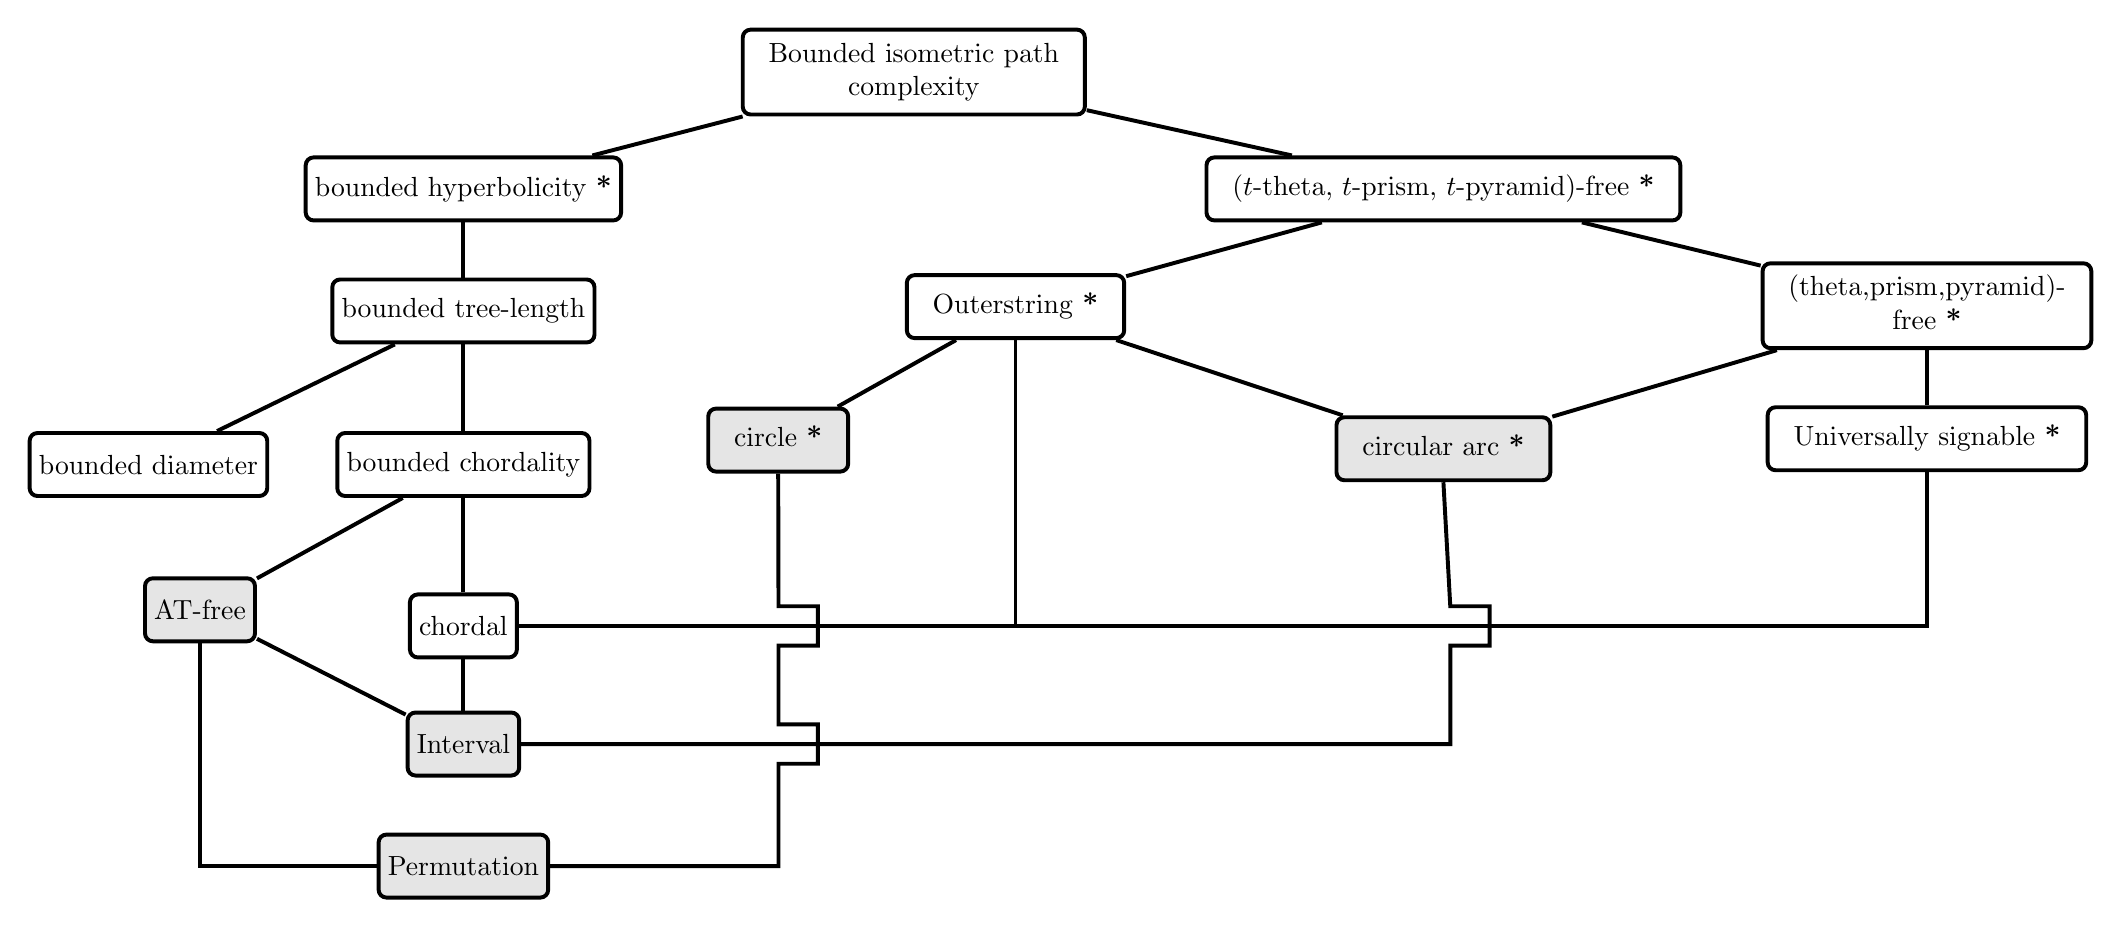
\begin{tikzpicture}[node distance=7mm]

\tikzstyle{mybox}=[fill=white,line width=0.5mm,rectangle, minimum height=.8cm,fill=white!70,rounded corners=1mm,draw];%[rectangle, minimum height=.8cm,fill=white!70,rounded corners=3mm,draw]
\tikzstyle{myedge}=[line width=0.5mm]
\newcommand{\tworows}[2]{\begin{tabular}{c}{#1}\\{#2}\end{tabular}}

     \node[mybox] (ipacc)  {\begin{tabular}{c}
          Bounded isometric path  \\
          complexity
     \end{tabular}};
     
     \node[mybox] (hyp) [below left=of ipacc,xshift=-1cm] {bounded hyperbolicity \textbf{*}} edge[myedge] (ipacc);
     
     
     
     \node[mybox] (theta) [below right=of ipacc,xshift=1cm] {\begin{tabular}{c}
          ($t$-theta, $t$-prism, $t$-pyramid)-free \textbf{*}
     \end{tabular}}  edge[myedge] (ipacc);
     
    \node[mybox] (outer) [below left=of theta,xshift=-0.5cm, yshift=-0.15cm] {\begin{tabular}{c}
          Outerstring \textbf{*} \\
          
     \end{tabular}} edge[myedge] (theta) ;
     
     \node[mybox, fill=gray!20] (circle) [below left=of outer,xshift=-0.2cm, yshift=-0.35cm] {\begin{tabular}{c}
          circle \textbf{*}
    \end{tabular}}  edge[myedge] (outer);
     
     
    \node[mybox] (truemper) [below right=of theta,xshift=0.5cm] {\begin{tabular}{c}
          (theta,prism,pyramid)-  \\
          free \textbf{*}
    \end{tabular}} edge[myedge] (theta) ;

     
     \node[mybox] (univ) [below =of truemper] {\begin{tabular}{c}
          Universally signable \textbf{*}
    \end{tabular}} edge[myedge] (truemper);
    
     \node[mybox] (treelength) [below=of hyp,] {bounded tree-length} edge[myedge] (hyp);
     
     \node[mybox] (chordality) [below=of treelength, yshift=-0.4cm] {bounded chordality} edge[myedge] (treelength);
  
     \node[mybox] (bdiameter) [below=of treelength, xshift=-4cm, yshift=-0.4cm] {bounded diameter} edge[myedge] (treelength);
     
    
    \node[mybox] (chordal) [below=of chordality, yshift=-0.5cm] {chordal} edge[myedge] (chordality); \draw[myedge] (chordal.east) -| (outer.south) ; \draw[myedge] (chordal.east) -| (univ.south) ;
     
    \node[mybox, fill=gray!20] (atfree) [below left=of chordality,xshift=-0.5cm, yshift=-0.5cm] {AT-free} edge[myedge] (chordality);
     
    \node[mybox, fill=gray!20] (interval) [below =of chordality,yshift=-2cm] {Interval} edge[myedge] (chordal) edge[myedge] (atfree); 

    
        
     \node[mybox, fill=gray!20] (arc) [below =of theta, yshift=-1.75cm] {\begin{tabular}{c}
          circular arc \textbf{*}
    \end{tabular} } edge[myedge] (outer) edge[myedge] (truemper);
    
    \draw[myedge] (interval.east) -- ++ (11.8,0) -- ++(0,1.25) -- ++ (0.5,0) -- ++ (0,0.5) -- ++ (-0.5,0) -- (arc.south);
    
    \node[mybox, fill=gray!20] (perm) [below =of interval] {Permutation}; \draw[myedge] (perm.west) -| (atfree.south); \draw[myedge] (perm.east) -- ++ (2.9,0) -- ++ (0, 1.3) -- ++ (0.5,0) -- ++ (0,0.5) -- ++ (-0.5,0) -- ++ (0,1) -- ++ (0.5,0) -- ++ (0,0.5) -- ++ (-0.5,0) -- (circle.south);
    
  \end{tikzpicture}}

\caption{Inclusion diagram for graph classes.
% discussed here (and related ones). 
If a class $A$ has an upward path to class $B$, then $A$ is included in $B$. Constant bounds for the isometric path complexity
% and constant-factor approximation algorithms for \IPC 
on graph classes marked with \textbf{*} are contributions of this paper.}
\label{fig:diagram}
\end{figure}


 \smallskip
 \noindent
\textbf{$\delta$-hyperbolic graphs:} A graph $G$ is said to be \emph{$\delta$-hyperbolic}~\cite{gromov1987} if for any four vertices $u,v,x,y$, the two larger of the three distance sums $\dist{u}{v}+\dist{x}{y}$, $\dist{u}{x}+\dist{v}{y}$ and $\dist{u}{y}+\dist{v}{x}$ differ by at most $2\delta$. A graph class $\mathcal{G}$ is \emph{hyperbolic} if there exists a constant $\delta$ such that every graph $G\in \mathcal{G}$ is $\delta$-hyperbolic. This parameter comes from geometric group theory and  was first introduced by Gromov~\cite{gromov1987} in order to study groups via their \emph{Cayley graphs}. The hyperbolicity of a tree is $0$, and in general, the hyperbolicity measures how much the distance function of a graph deviates from a tree metric.   Many structurally defined graph classes like chordal graphs, \emph{cocomparability} graphs~\cite{corneil2013ldfs}, \emph{asteroidal-triple free} graphs~\cite{corneil1997asteroidal}, graphs with bounded \emph{chordality} or \emph{treelength} are hyperbolic~\cite{chepoi2008diameters,kosowski2015k}. Moreover, hyperbolicity has been found to capture important properties of several large practical graphs such as the Internet graph~\cite{shavitt2004curvature} or database relation graphs~\cite{walter2002interactive}. Due to its importance in discrete mathematics, algorithms, \emph{metric graph theory}, researchers have studied various algorithmic aspects of hyperbolic graphs~\cite{chepoi2008diameters,coudert2021enumeration,chepoi2017core,das2018effect}. Note that graphs with diameter~2 are hyperbolic, which may contain any graph as an induced subgraph.

 \smallskip
\noindent
\textbf{(theta, prism, pyramid)-free graphs:} A \emph{theta} is a graph made of three vertex-disjoint induced paths $P_1 = a\ldots b$, $P_2 = a\ldots b$, $P_3 = a\ldots b$ of lengths at least~2, and such that no edges exist between the paths except the three edges incident to $a$ and the three edges incident to $b$. 
% See Figure~\ref{fig:struct} for an illustration. 
A \emph{pyramid} is a graph made of three induced paths $P_1 = a\ldots b_1$, $P_2 = a\ldots b_2$, $P_3 = a\ldots b_3$, two of which have lengths at least $2$, vertex-disjoint except at $a$, and such that $b_1 b_2 b_3$ is a triangle and no edges exist between the paths except those of the triangle and the three edges incident to $a$. A \emph{prism} is a graph made of three vertex-disjoint induced paths $P_1 = a_1\ldots b_1$, $P_2 = a_2\ldots b_2$, $P_3 = a_3\ldots b_3$ of lengths at least $1$, such that $a_1 a_2 a_3$ and $b_1 b_2b_3$ are triangles and no edges exist between the paths except those of the two triangles. A graph $G$ is \emph{(theta, pyramid, prism)}-free if $G$ does not contain any induced subgraph isomorphic to a theta, pyramid or prism. A graph is a \emph{$3$-path configuration} if it is a theta, pyramid or prism. The study of $3$-path configurations dates back to the works of Watkins and Meisner~\cite{watkins1967cycles} in 1967 and plays ``special roles'' in the proof of the celebrated \emph{Strong Perfect Graph Theorem}~\cite{chudnovsky2006strong,diot2020theta,trotignon2013perfect,vuskovic2013world}. Important graph classes like chordal graphs, \emph{circular arc} graphs, \emph{universally-signable} graphs~\cite{conforti1997universally} exclude all $3$-path configurations. Popular graph classes like \emph{perfect} graphs, \emph{even hole}-free graphs exclude some of the $3$-path configurations. Note that, (theta, prism, pyramid)-free graphs are not hyperbolic. To see this, consider a cycle $C$ of order $n$. Clearly, $C$ excludes all $3$-path configurations and has hyperbolicity $\Omega(n)$.



 \smallskip
 \noindent
\textbf{Outerstring graphs:} A set $S$ of simple curves on the plane is \emph{grounded} if there exists a horizontal line containing one endpoint of each of the curves in $S$. A graph $G$ is an \emph{outerstring} graph if there is a collection $C$ of grounded simple curves and a bijection between $V(G)$ and $C$ such that two curves in $S$ intersect if and only if the corresponding vertices are adjacent in $G$. 
% See Figure~\ref{fig:struct}(d) for an illustration. 
The term ``outerstring graph'' was first used in the early 90's~\cite{kratochvil1991string} in the context of studying intersection graphs of simple curves on the plane. Many well-known graph classes like chordal graphs, \emph{circular arc} graphs~\cite{francis2014forbidden}, \emph{circle} graphs (intersection graphs of chords of a circle~\cite{davies2021circle}), or cocomparability graphs~\cite{corneil2013ldfs} are also outerstring graphs and thus, motivated researchers from the \emph{geometric graph theory} and \emph{computational geometry} communities to study algorithmic and structural aspects of outerstring graphs and its subclasses~\cite{biedl2018size,bose2022computing,cardinal2017intersection,keil2017algorithm,rok2019outerstring}. Note that, in general, outerstring graphs may contain a prism, pyramid or theta as an induced subgraph. Moreover, cycles of arbitrary order are outerstring graphs, implying that outerstring graphs are not hyperbolic.

\smallskip

 It is clear from the above discussion that the classes of hyperbolic graphs, (theta, prism, pyramid)-free graphs, and outerstring graphs are {pairwise} incomparable (with respect to the containment relationship). We show that the isometric path complexities of all the above graph classes are small.

\subsection{Our contributions}


The main technical contribution of this paper are as follows. First we prove that the isometric path complexity can be computed in polynomial time.

\begin{theorem}
    \label{thm:ipcoInP}
    Given a graph $G$ with $n$ vertices and $m$ edges, it is possible to compute $\ipco{G}$ in $O(n^2m)$ time.
\end{theorem}

Recall that, the above theorem and Lemma~\ref{lem:ipac-ipco} imply that for any undirected graph $G$, $\ipac{G}$ can be computed in polynomial time. Then we show that the isometric path complexity remains bounded on hyperbolic graphs, (theta, pyramid, prism)-free graphs, and outerstring graphs. Specifically, we prove the following theorem.

\begin{theorem}\label{thm:main}
Let $G$ be a graph.
\vspace{-5pt}
    \begin{enumerate}[label=(\alph*)]
        \item \label{thm:hyperbolicity} If the hyperbolictiy of $G$ is at most $\delta$, then $\ipco{G} \leq  4\delta+3$.
        \item\label{thm:truemper} If $G$ is a (theta, pyramid, prism)-free graph, then $\ipco{G} \leq 71$.
        \item\label{thm:outer} If $G$ is an outerstring graph, then $\ipco{G} \leq 95$.
    \end{enumerate}
\end{theorem}

To the best of our knowledge, the isometric path complexity being bounded (by constant(s)) is the only known non-trivial property shared by any two or all three of these graph classes. Theorem~\ref{thm:main} shows that isometric path complexity (equivalently isometric path antichain cover number), as recently introduced graph parameters, are general enough to unite these three graph classes by their metric properties. We hope that this definition will be useful for the field of metric graph theory, for example by enabling us to study (theta,prism,pyramid)-free graphs and outerstring graphs from the perspective of metric graph theory. 

We provide a unified proof for Theorem~\ref{thm:main}\ref{thm:truemper} and~\ref{thm:main}\ref{thm:outer} by proving that the isometric path complexity of \emph{($t$-theta, $t$-pyramid, $t$-prism)}-free graphs~\cite{trotignonprivate} (see Section~\ref{sec:main} for a definition) is bounded by a linear function of $t$. Due to the above theorems, we also have as corollaries that there is a {polynomial-time} approximation algorithm for \IPC with approximation ratio
\begin{enumerate*}[label=(\alph*)]
    \item $4\delta+3$ on $\delta$-hyperbolic graphs,
    \item $73$ on (theta, prism, pyramid)-free graphs,
    \item $95$ on outerstring graphs, and
    \item $8t+63$ on ($t$-theta, $t$-pyramid, $t$-prism)-free graphs.
\end{enumerate*}



To contrast with Theorem~\ref{thm:main}, we construct highly structured graphs with small \emph{treewidth} and large isometric path complexity. A \emph{wheel} consists of an induced cycle $C$ of order at least $4$ and a vertex $w \notin V(C)$ adjacent to at least three vertices of $C$. The three path configurations introduced earlier and the wheel together are called \emph{Truemper configurations}~\cite{vuskovic2013world} and they are important objects of study in structural and algorithmic graph theory~\cite{aboulker2015wheel,diot2020theta}. 


\begin{theorem}\label{thm:lower}
For every $k\geq 1$, 
\vspace{-7.5pt}
\begin{enumerate}[label=(\alph*)]
    \item\label{it:a} there exists a (pyramid, prism, wheel)-free graph $G$ with tree-width $2$, hyperbolicity at least $\lceil\frac{k}{2}\rceil-1$ and $\ipco{G}\geq k$;
    \item\label{it:b} there exists a (theta, prism, wheel)-free planar graph $G$ with tree-width at most $3$, hyperbolicity at least $\lceil\frac{k}{2}\rceil-1$ and $\ipco{G}\geq k$;
    \item\label{it:c} there exists a (theta, pyramid, wheel)-free planar graph $G$ with hyperbolicity at least $\lceil\frac{k}{2}\rceil-1$ and $\ipco{G}\geq k$;
    \item \label{it:d} { there exists a (prism, pyramid, wheel)-free planar bipartite graph $G$ such that $|V(G)|$ is $O(k^2)$, $G$ has an isometric path cover of size $3k+1$ and any $v$-rooted isometric path cover of $G$ has cardinality at least $k^2$ for any $v\in V(G)$. }
\end{enumerate}
\end{theorem}

 {  
Theorem~\ref{thm:lower}\ref{it:d} proves that the approximation algorithm for \textsc{Isometric Path Cover} proposed by Chakraborty et al.~\cite{ChakrabortyD0FG22} cannot provide a $o(\sqrt{n})$ approximation ratio (even if the inputs are restricted to planar bipartite graphs of order $n$). Note that previous known lower bound (stated in~\cite{ChakrabortyD0FG22}) was $o(\sqrt{\log n})$.}

\smallskip

%A short version of this paper (missing full proofs and other material) appeared in the prooceedings of the MFCS 2023 conference~\cite{shortversion}.
%
%\smallskip

 \noindent \textbf{Organisation.} In Section~\ref{sec:prelim}, we recall some definitions and some results. In Section~\ref{sec:ipcoInP}, we present an algorithm to compute the isometric path complexity of a graph and prove Theorem~\ref{thm:ipcoInP}. In Section~\ref{sec:main}, we prove Theorem~\ref{thm:main}. In Section~\ref{sec:lower}, we prove Theorem~\ref{thm:lower}. We conclude in Section~\ref{sec:conclu}.





\section{Definitions and preliminary observations}\label{sec:prelim}

In this section, we recall some definitions and some related observations. A sequence of distinct vertices forms a \emph{path} $P$ if any two consecutive vertices are adjacent. 
Whenever we fix a path $P$ of $G$, we shall refer to the subgraph formed by the edges between the consecutive vertices of $P$. The \emph{length} of a path $P$, denoted by $|P|$, is the number of its vertices minus  one. A path is \emph{induced} if there are no graph edges joining non-consecutive vertices. A path is \emph{isometric} if it is a shortest path between its endpoints.  For two vertices $u,v$ of a graph $G$, $\dist{u}{v}$ denotes the length of an isometric path between $u$ and $v$. 

{In a directed graph, a \emph{directed path} is a path in which all arcs are oriented in the same direction.} For a path $P$ of a graph $G$ between two vertices $u$ and $v$, the vertices $V(P)\setminus \{u,v\}$ are \emph{internal vertices} of $P$. A path between two vertices $u$ and $v$ is called a $(u,v)$-path.  Similarly, we have the notions of \emph{isometric $(u,v)$-path} and \emph{induced $(u,v)$-path}. The interval $I(u,v)$ between two vertices $u$ and $v$ consists of all vertices that belong to an isometric $(u,v)$-path. For a vertex $r$ of $G$ and a set $S$ of vertices of $G$, the \emph{distance of $S$ from $r$}, denoted as $\dist{r}{S}$, is the minimum of the distance between any vertex of $S$ and $r$. For a subgraph $H$ of $G$, the \emph{distance of $H$ w.r.t. $r$} is $\dist{r}{V(H)}$. Formally, we have $\dist{r}{S}=\min\{\dist{r}{v}\colon v\in  S\}$ and $\dist{r}{H}=\dist{r}{V(H)}$.  

 For a graph $G$ and a vertex $r \in V(G)$, consider the following operations on $G$. First, remove all edges $xy$ from $G$ such that $\dist{r}{x}=\dist{r}{y}$. Let $G'_r$ be the resulting graph. Then, for each edge $e=xy\in E(G'_r)$ with $\dist{r}{x} = \dist{r}{y} - 1$, orient $e$ from $y$ to $x$. Let $\overrightarrow{G_r}$ be the directed acyclic graph formed after applying the above operation on $G'$. Note that this digraph can easily be computed in linear time using a Breadth-First Search (BFS) traversal with starting vertex $r$. 
 
{  The known approximation algorithm for \IPC from~\cite{ChakrabortyD0FG22} can now be stated as follows: $(i)$ For each vertex $r\in V(G)$, compute $\overrightarrow{G_r}$ and find a minimum path cover $\mathcal{C}_r$ of $\overrightarrow{G_r}$, and then $(ii)$ report a $\mathcal{C}_r$ with minimum cardinality. {The following definition is inspired by the terminology of posets (as the graph $\overrightarrow{G_r}$ can be seen as the Hasse diagram of a poset) and will be useful to analyze the above algorithm.}}

\begin{definition}\label{D:acSet}
\sloppy For a graph $G$ and a vertex $r\in V(G)$, two vertices $x,y\in V(G)$ are \emph{antichain vertices} if there are no directed paths from $x$ to $y$ or from $y$ to $x$ in $\overrightarrow{G_r}$. A set $X$ of vertices of $G$ is an \emph{antichain set} if any two vertices in $X$ are antichain vertices. 
\end{definition}


\begin{definition}[{\cite{ChakrabortyD0FG22}}]\label{D:acWidth}
Let $r$ be a vertex of a graph $G$. For a subgraph $H$, $\anticp{r}{H}$ shall denote the maximum antichain set of $H$ in $\overrightarrow{G_r}$. The \emph{isometric path antichain cover number} of $\overrightarrow{G_r}$, denoted by $\ipac{\overrightarrow{G_r}}$, is defined as follows: \[\ipac{\overrightarrow{G_r}}=\max\left\{|\anticp{r}{P}|\colon~P~\text{is an isometric path}\right\}.\]
The \emph{isometric path antichain cover number} of graph $G$, denoted as $\ipac{G}$, is defined as the minimum over all possible antichain covers of its associated directed acyclic graphs: \[\ipac{G}=\min \left\{\ipac{\overrightarrow{G_r}}\colon r\in V(G)\right\}.\]
\end{definition}

For technical purposes, we also introduce the following definition. For a graph $G$ and a vertex $r$ of $G$, let $\ipcor{r}{G}$ denote the minimum integer $k$ such that any isometric path $P$ of $G$ can be covered by $k$ $r$-rooted isometric paths (The notation reflects that it is a dual notion of $\ipac{\overrightarrow{G_r}}$). Using Dilworth's Theorem we prove the following important lemma.


\begin{lemma}\label{lem:ipac-ipco}
    For any graph $G$ and vertex $r$, $\ipcor{r}{G} = \ipac{\overrightarrow{G_r}}$. Therefore,  $\ipco{G}=\ipac{G}$.
\end{lemma}

\begin{proof}
Let $r$ be a vertex of $G$ such that any isometric path of $G$ can be
covered by $\ipcor{r}{G}$ $r$-rooted isometric paths. Let $P$ be an
arbitrary isometric path of $G.$ Since two vertices of an antichain of
$\overrightarrow{G_r}$ cannot be covered by a single $r$-rooted path and
$P$ is covered by $\ipcor{r}{G}$ $r$-rooted path, we deduce $|\anticp{r}{P}|\le
\ipcor{r}{G}$. This is true for any isometric path $P$ of $G$. Hence,
$ \ipac{\overrightarrow{G_r}} \leq \ipcor{r}{G}$. Conversely, consider a vertex $r\in V(G).$ By definition of $\ipcor{r}{G}$,
there is an isometric path $P$ that cannot be covered by $(\ipcor{r}{G}-1)$
$r$-rooted isometric paths. By Dilworth theorem, $P$ contains an
antichain of $\overrightarrow{G_r}$ of size $\ipcor{r}{G}.$ Hence
$|A_r(P)|\geq \ipcor{r}{G}$ and $\ipac{\overrightarrow{G_r}}\geq \ipcor{r}{G}$.
The second part of the lemma follows immediately.
% Since this is true for any vertex $r$ we get $\ipac{G}\ge \ipco{G}$.
\end{proof}

We also recall the following theorem and proposition from~\cite{ChakrabortyD0FG22}. 

\begin{theorem}[\cite{ChakrabortyD0FG22}]\label{thm:ipac-approx}
For a graph $G$, if $\ipac{G} \leq c$, then \IPC admits a {polynomial-time} $c$-approximation algorithm on $G$.
% \todo{F: why is this not a theorem?} \todo{D: I usually use proposition to state existing results. But we can use Theorem too.}\todo{F: I find that strange. Previous work has to be acknowledged properly. Usually "Proposition" means it's a minor and/or easy-to-prove result.}
\end{theorem}


% We also recall the proof of the following proposition which will be used heavily in this paper.

\begin{proposition}[\cite{ChakrabortyD0FG22}]\label{prp:antichain-length}
Let $G$ be a graph and $r$, an arbitrary vertex of $G$. Consider the directed acyclic graph $\overrightarrow{G_r}$, and let $P$ be an isometric path between two vertices $x$ and $y$ in $G$. Then $|P|\geq |\dist{r}{x}-\dist{r}{y}| + |\anticp{r}{P}| - 1$. 
% \todo{F: I suggest we reproduce the proof (perhaps in an appendix for a conf submission), since this is quite crucial.}
\end{proposition}

\begin{proof}
Orient the edges of $P$ from $y$ to $x$ in $G$. First, observe that $P$ must contain a set $E_1$ of oriented edges such that $|E_1|=|\dist{r}{y}-\dist{r}{x}|$ and for any $\overrightarrow{ab}\in E_1$, $\dist{r}{a}=\dist{r}{b}+1$. Let the vertices of the largest antichain set of $P$ in $\overrightarrow{G_r}$, \ie, $\anticp{r}{P}$, be ordered as $a_1,a_2,\ldots,a_t$ according to their occurrence while traversing $P$ from $y$ to $x$. For $i\in [2,t]$, let $P_i$ be the subpath of $P$ between $a_{i-1}$ and $a_i$. Observe that for any $i\in [2,t]$, since $a_i$ and $a_{i-1}$ are antichain vertices, there must exist an oriented edge $\overrightarrow{b_ic_i}\in E(P_i)$ such that either $\dist{r}{b_i} = \dist{r}{c_i}$ or $\dist{r}{b_i}=\dist{r}{c_i} - 1$. Let $E_2=\{b_ic_i\}_{i\in [2,t]}$. Observe that $E_1\cap E_2=\emptyset$ and therefore $|P|\geq |E_1| + |E_2| = |\dist{r}{y}-\dist{r}{x}| + |\anticp{r}{P}| - 1$.
\end{proof}    



%  \begin{observation}\label{obs:dist-same-level}
%  Let $G$  be a graph and $r$ be an arbitrary vertex of $G$. Let $P$ be an isometric $(u,v)$-path in $G$ such that $\dist{r}{u}\leq \dist{r}{v}$. Let $w$ be a vertex with $\dist{r}{u}=\dist{r}{w}$ such that $w$ lies in an oriented $(r,v)$-path in $\overrightarrow{G_r}$. If $|\anticp{r}{P}|\geq \alpha$, then $\dist{u}{w}\geq \alpha - 1$. \todo{F: is this really an "observation"? It relies on Prop.~\ref{prp:antichain-length}, but normally "observation" is a very easy thing to observe. And in fact, it is never cited in the paper. Is it really needed? \dd{I think, this observation is not used. Therefore, I am commenting it.}}
%  \end{observation}
%  \begin{proof}
%  If $w=v$, then the statement is trivially true. Otherwise, due to Proposition~\ref{prp:antichain-length} we have that $\dist{u}{v} \geq \dist{r}{v} - \dist{r}{u} + \alpha - 1$. If $\dist{u}{w}\leq \alpha - 2$ then $\dist{u}{v} \leq \dist{u}{w} + \dist{w}{v} \leq \alpha-2 + \dist{r}{v} - \dist{r}{u}$, a contradiction.
% \end{proof}

% \subsection{Some useful lemma}



% In this section, we prove some basic observations about (theta, pyramid,prism)-free graphs for completeness.






% \begin{observation}
% Let $G$ be a graph with an induced cycle $C$ of order at least $4$. Let $P$ be an induced $(u,v)$-path of length such that $u,v$ $N[P]\cap V(C) \neq \emptyset$ and  such that the following conditions hold:
% \begin{enumerate}
%     \item $P$ contains a subpath $P'$ of length at least $2$ such that no internal vertex of $P'$ vertex $z\in V(C)$ and 
% \end{enumerate}
% \end{observation}
% Lemma~\ref{lem:dil} also provides a Gallai-Millgram~\cite{gallai1960} type upper bound for \IPC. 

% \subsection{Lemmas on the isometric path antichain cover number}

% In this section, we shall prove some lemmas relating the isometric path antichain cover number with other parameters. 






% Next, we shall relate isometric path antichain cover number with a parameter called \emph{cluster diameter}, introduced in~\cite{dourisboure2007tree}. Let $G$ be a graph and $r$ be an arbitrary vertex of $G$. For a non-negative integer $i$, let $G^i(r)$ denote the graph induced by the vertices whose distance from $r$ is at least $i$. Formally, $G^i(r)=G[\{u\colon \dist{r}{u}\geq i\}]$. A \emph{cluster} is a set $S$ of vertices such that all vertices of $S$ are at the same distance from $r$ and any two vertices of $S$ lie in the same connected component of $G^i(r)$, where $i=\dist{r}{S}$.  The \emph{cluster diameter of $G$ with respect to $r$}, denoted as $\cdiam{r}{G}$, was defined in~\cite{dourisboure2007tree} as follows: $$\cdiam{r}{G} = \max\{\dist{u}{v}\colon u,v~\text{lie in the same cluster with respect to }r \}$$


% \begin{proposition}[\cite{chakraborty2022}]\label{prp:heavyness}
%   Let $G$ be a graph, $r$ be an arbitrary vertex of $G$, and let $P$ be an isometric path such that $|\anticp{r}{P}| \geq \alpha$ in $\overrightarrow{G_r}$. Then $\cdiam{r}{G}\geq \left\lceil\frac{\alpha}{2}\right\rceil - 1$.
% \end{proposition}


% Next, we state the following definition.

% \begin{definition}
%  For an integer $t\geq 1$, a graph $G$ is \emph{$t$-slender} if there exists a vertex $r\in V(G)$ such that, for all vertices $u,v\in V(G)$ with $\dist{r}{u}=\dist{r}{v}$, we have $\dist{u}{v}\leq t$.
% %  \todo{F: again, why use $w$ and not $v$?}
% \end{definition}

% \begin{proposition}[\cite{chakraborty2022}]\label{prp:c-slender}
% Let $G$ be a $t$-slender graph for some integer $t\geq 1$. Then, $\ipac{G} \leq t+1$.
% \end{proposition}

% \section{Proof of Theorem~\ref{thm:approx-IPC}}\label{sec:alternate-def}




% Lemma~\ref{lem:ipac-ipco} and Theorem~\ref{thm:ipac-approx} imply Theorem~\ref{thm:approx-IPC}.

\section{Proof of Theorem \ref{thm:ipcoInP}} \label{sec:ipcoInP}


In this section we provide a polynomial-time algorithm to compute the
isometric path complexity of a graph. Let $G$ be a graph.  In the
following lemma, we provide a necessary and sufficient condition for
two vertices of an isometric path to be covered by the same isometric
$r$-rooted path in $\overrightarrow{G_r}$ for some vertex $r\in V(G)$.

\begin{lemma}\label{lemma1}
  Let $r$ be vertex of $G$. If $P=(u=v_0,\dots,v_k=v)$ is an isometric
  $(u,v)$-path with $\dist{r}{u}\le \dist{r}{v}$ then there exists an
  isometric $r$-rooted path containing $u, v$ in
  $\overrightarrow{G_r}(P)$ if and only if
  $\dist{v_{i+1}}{r} = \dist{v_i}{r}+1$ for all
  $i\in \{0,\dots,k-1\}.$
\end{lemma}

% (Proofs of Lemmas, Observations and Claims marked with (*) can be found
% in the Appendix.) % In the next section, we introduce some notations
% that will be used to describe the algorithm and prove its correctness.

\begin{proof}
  If $\dist{v_{i+1}}{r}= \dist{v_i}{r}+1$ for every
  $i\in \{0,\dots,k-1\}$ then the path obtained by concatenating an
  isometric $(r,u)$-path and the path $P$ is an isometric $r$-rooted
  $(r,v)$-path containing $u, v$ in $\overrightarrow{G_r}(P)$.  Now
  suppose that there exists an isometric $r$-rooted path containing
  $u, v$ in $\overrightarrow{G_r}(P)$, \ie,
  $\dist{r}{v}-\dist{r}{u}=\dist{u}{v}.$ Then, along any path from $u$
  to $v$, we need to traverse at least $\dist{u}{v}$ edges increasing
  the distance to $r$. Since $P$ is an isometric $(u,v)$-path, it
  contains exactly $\dist{u}{v}$ edges. Hence,
  $\dist{r}{v_{i+1}}=\dist{r}{v_i}+1$ for every
  $i\in \{0,\dots,k-1\}$.
\end{proof}

\subsection{Notations and preliminary observations}


We now introduce some notations that will be used to describe the
algorithm and prove its correctness.  Consider three vertices $r,x,v$
of $G$ such that $x \neq v$. Let $\pathseta{r}{x}{v}$ denote the set
of all isometric $(x,v)$-paths $P$ containing a vertex $u$ that is
adjacent to $v$ and satisfies
$\dist{r}{u}=\dist{r}{v}-1$. Analogously, let $\pathseteq{r}{x}{v}$
denote the set of all isometric $(x,v)$-paths $P$ containing a vertex
$u$ that is adjacent to $v$ and satisfies $\dist{r}{u}=\dist{r}{v}$
and let $\pathsetd{r}{x}{v}$ denote the set of all isometric
$(x,v)$-paths $P$ containing a vertex $u$ that is adjacent to $v$ and
satisfies $\dist{r}{u}=\dist{r}{v}+1$. Observe that the set of
isometric $(x,v)$-paths is precisely
$\pathseta{r}{x}{v} \cup \pathseteq{r}{x}{v} \cup \pathsetd{r}{x}{v}$
and that some of these sets may be empty.

Given a path $P$, we denote by $|\coverP{r}{P}|$ the minimum size of a
set of isometric $r$-rooted paths covering the vertices of $P$.  We
denote by $\gamma^r_{\searrow}(x,v)$ and $\beta^r_{\searrow}(x,v)$
respectively the minimum of $|\coverP{r}{P}|$ and
$|\coverP{r}{P-\{v\}}|$ over all paths $P\in \pathseta{r}{x}{v}$. More
formally,
\begin{align*}
  \gamma^r_{\searrow}(x,v)&=\max\left\{ |\coverP{r}{P}| \colon P \in \pathseta{r}{x}{v} \right\}, \\
  \beta^r_{\searrow}(x,v)&=\max\left\{ |\coverP{r}{P - \{v\}}|\colon P\in \pathseta{r}{x}{v} \right\}.
\end{align*}
%
Note that if $\pathseta{r}{x}{v}$ is empty, we have
$\gamma^r_{\searrow}(x,v) = \beta^r_{\searrow}(x,v) = 0$.  We define
similarly $\gamma^r_{\nearrow}(x,v)$, $\beta^r_{\nearrow}(x,v)$, and
$\gamma^r_{\rightarrow}(x,v)$:
\vspace{-7.5pt}
\begin{align*}
  \gamma^r_{\nearrow}(x,v)&=\max\left\{ |\coverP{r}{P}|\colon P\in \pathsetd{r}{x}{v} \right\},\\ 
  \beta^r_{\nearrow}(x,v)&=\max\left\{ |\coverP{r}{P- \{v\}}|\colon P\in \pathsetd{r}{x}{v} \right\},\\
  \gamma^r_{\rightarrow}(x,v)&=\max\left\{ |\coverP{r}{P}|\colon P\in \pathseteq{r}{x}{v} \right\}. %
  % \beta^r_{\rightarrow}(x,v)&=\max\left\{ |\coverP{r}{P- \{v\}}|\colon P\in \pathseteq{r}{x}{v} \right\} \\
\end{align*}
%
Finally, let
$\gamma^r(x,v) = \max\left\{ \gamma^r_{\searrow}(x,v),
  \gamma^r_{\rightarrow}(x,v) , \gamma^r_{\nearrow}(x,v) \right\} $ be
the maximum of $|S_r(P)|$ over all isometric $(x,v)$-paths $P$.
%
In our algorithm, we will need also to consider the case where $v=x$
as an initial case. For practical reasons, we let
$\gamma^r(x,x) = \gamma^r_{\searrow}(x,x) =
\gamma^r_{\rightarrow}(x,x) = \gamma^r_{\nearrow}(x,x) = 1$ and
$\beta^r_{\searrow}(x,x) = \beta^r_{\nearrow}(x,x) =0$.
Based on the above notations and Lemma~\ref{lem:ipac-ipco}, we have the following observation.

\begin{observation}\label{obs:triv-poly}
  For any graph $G$ and any vertex $r$ of $G$, we have
  $\ipco{\overrightarrow{G_r}} = \ipac{\overrightarrow{G_r}} =
  \max_{x,v} \gamma^r(x,v)$ and
  $\ipco{G} = \ipac{G} = \min_{r} \max_{x,v} \gamma^r(x,v)$.
\end{observation}

Observation~\ref{obs:triv-poly} implies that to compute the isometric
path complexity of a graph it is enough to compute the parameter
$\gamma^r(x,v)$ for all $r,x,v\in V(G)$ in polynomial time. In the
next section, we focus on achieving this goal without computing
explicitly any of the sets $\pathseta{r}{x}{v}$, $\pathseteq{r}{x}{v}$
or $\pathsetd{r}{x}{v}$. (Note that the size of these sets could be
exponential in the number of vertices of the graph).




\subsection{An algorithm to compute \boldmath{$\gamma^r(x,v)$}}

Throughout this section, let $r$ and $x$ be two fixed vertices of $G$. We shall call $r$ as the ``root'' and $x$ as the ``source'' vertex. The objective of this section is to compute the parameter $\gamma^r(x,v)$ for all vertices $v\in V(G)$. 

In the sequel, since we always refer to a fixed root $r$ and source
$x$, we omit $r$ and $x$ and use the shorthand $\gamma(v)$ for
$\gamma^r(x,v).$ We do the same with the notations
$\gamma_{\nearrow}(v)$, $\gamma_{\rightarrow}(v)$,
$\gamma_{\searrow}(v)$, $\beta_{\nearrow}(v)$, and
$\beta_{\searrow}(v)$ that also refer to fixed vertices $r$ and
$x$
In the following lemmas, we shall provide explicit (recursive)
formulas to compute $\gamma_{\nearrow}(v)$, $\gamma_{\rightarrow}(v)$,
$\gamma_{\searrow}(v)$, $\beta_{\nearrow}(v)$, and
$\beta_{\searrow}(v)$. Using these formulas, we will show how to
compute $\gamma(v)$ for all $v\in V(G)$ in a total of
$O(|E(G)|)$-time.

% \subsubsection{Important lemmas}


\begin{observation}\label{lem:beta-arrow}
  If $r$ is the root vertex, $x$ the source vertex, and $v$ is
  distinct from $x$, then
  % Let $r$ be the root vertex, $x$ be the source vertex, and $v$ a
  % vertex distinct from $x$. Then
  \begin{align*}
    \beta_{\searrow}(v) &= \max \{ \gamma(u) : u\in I(x,v) \cap N(v);\
                          \dist{r}{u}=\dist{r}{v}-1 \},\\
    % \beta_{\rightarrow}(v) &= \max \{ \gamma(u) : u\in I(x,v) \cap N(v);\
    %                       \dist{r}{u}=\dist{r}{v} \},\\
    \beta_{\nearrow}(v) &= \max \{ \gamma(u) : u\in I(x,v) \cap N(v);\
                          \dist{r}{u}=\dist{r}{v}+1 \}.
  \end{align*}
\end{observation}

% \begin{proof}
%   Consider a path $P \in \pathseta{r}{x}{v}$ such that
%   $\beta_{\searrow}(v) = \coverP{r}{P - \{v\}}$ and let $u$ be the
%   neighbour of $v$ on $P$. Note that $\dist{r}{u}=\dist{r}{v}-1$. Since
%   $P - \{v\}$ is an isometric $(x,u)$-path, we have
%   $\beta_{\searrow}(v) = \coverP{r}{P - \{v\}} \leq \gamma(u) \leq
%   \max \{ \gamma(u') : u'\in I(x,v) \cap N(v);\
%   \dist{r}{u'}=\dist{r}{v}-1 \}$. Conversely, consider a vertex $u$
%   such that
%   $\gamma(u) = \max \{ \gamma(u') : u'\in I(x,v) \cap N(v);\
%   \dist{r}{u'}=\dist{r}{v}-1 \}$ and let $P'$ be an isometric
%   $(x,u)$-path $P'$ such that $\gamma(u) =\coverP{r}{P'}$. Then the
%   path obtained by appending $v$ to $P'$ belongs to
%   $\pathseta{r}{x}{v}$, and thus
%   $\gamma(u) =|\coverP{r}{P'}| \leq \beta_{\searrow}(v)$.

%   The proof of the other case is similar. 
% \end{proof}

% Similar arguments as Lemma~\ref{lem:beta-searrow} proves the following two lemma.

% \begin{lemma}\label{lem:beta-rightarrow}
%     Let $v$ be a vertex of $G$, $r$ be the root vertex and $x$ be the source vertex. Then $\beta_{\rightarrow}(v) = \max \{ \gamma(u) : u\in I(x,v) \cap N(v),\  \dist{r}{u}=\dist{r}{v} \}$. 
% \end{lemma}

% \begin{lemma}\label{lem:beta-nearrow}
%     Let $v$ be a vertex of $G$, $r$ be the root vertex and $x$ be the source vertex. Then $\beta_{\nearrow}(v) = \max \{ \gamma(u) : u\in I(x,v) \cap N(v),\  \dist{r}{u}=\dist{r}{v}+1 \}$. 
% \end{lemma}
 

\begin{lemma}\label{lem:gamma-rightarrow}
  If $r$ is the root vertex, $x$ the source vertex, and $v$ is
  distinct from $x$, then
  $\gamma_{\rightarrow}(v) = \max \{ 1+\gamma(u) : u\in I(x,v) \cap
  N(v);\ \dist{r}{u}=\dist{r}{v} \}$.
\end{lemma}


\begin{proof}
  % Suppose first that $v$ is adjacent to $x$. Then $P = (x,v)$ is the
  % unique isometric $(x,v)$-path.  If $\dist{r}{x} \neq \dist{r}{v}$,
  % then $ \gamma_{\rightarrow}(v) = 0$ since
  % $\pathseteq{r}{x}{v} = \emptyset$.  Since the set
  % $\{u\in I(x,v) \cap N(v);\ \dist{r}{u}=\dist{r}{v} \}$ is also
  % empty, the statement holds. If $\dist{r}{x} = \dist{r}{v}$, then
  % $\gamma_{\rightarrow}(v) = |\coverP{r}{P}| = 2 = 1 +\gamma(x)$ and
  % we are done.
  Observe that $\pathseteq{r}{x}{v}$ is empty if and only if there is
  no vertex $u\in I(x,v) \cap N(v)$ such that
  $\dist{r}{u}=\dist{r}{v}$. If $\pathseteq{r}{x}{v}$ is empty, then
  $\gamma_{\rightarrow}(v) =0$ and we are done.
  
  % Assume now that $v$ is not adjacent to $x$.
  Suppose now that $\pathseteq{r}{x}{v} \neq \emptyset$.  Let
  $P=(x=v_0,\dots,v_{i-1},v_i=v)$ be a path such that
  $|\coverP{r}{P}| = \gamma_{\rightarrow}(v)$. Observe that
  $\dist{r}{v_{i-1}}=\dist{r}{v_i}$.  Let $Q = (v_0,\dots,v_{i-1})$
  and consider a set $S$ of isometric $r$-rooted paths covering the
  vertices of $Q$ of size $|\coverP{r}{Q}|$ and a $(r,v_i)$-shortest
  path $P_i$. Observe that $S \cup \{P_{i}\}$ is a set of isometric
  $r$-rooted paths covering the vertices of $P$. Consequently
  $\gamma_{\rightarrow}(v_i) = |\coverP{r}{P}| \leq |\coverP{r}{Q}|+1
  \leq \gamma(v_{i-1})+1$.

  Consider now an isometric $(x,v_{i-1})$-path $Q'$ such that
  $\gamma(v_{i-1}) = |\coverP{r}{Q'}|$. Let $P'$ be the isometric
  $(x,v_i)$-path obtained by appending $v_i$ to $Q'$. Consider a set
  $S'$ of isometric $r$-rooted paths covering the vertices of $P'$ of
  size $|\coverP{r}{P'}|$ and let $P_i' $ be a path of $S'$ covering
  $v_i$.  By Lemma~\ref{lemma1}, no vertex of $Q'$ is covered by
  $P_i'$. Consequently, $S'\setminus \{P_i'\}$ is a set of isometric
  $r$-rooted paths covering all vertices of $Q'$ and thus
  $\gamma(v_{i-1}) \leq |\coverP{r}{P'}| -1 \leq
  \gamma_{\rightarrow}(v_i) -1$. Thus, we have
  $\gamma_{\rightarrow}(v_i) = \gamma(v_{i-1}) +1$.
\end{proof}

\begin{lemma}\label{lem:gamma-searrow}
  If $r$ is the root vertex, $x$ the source vertex, and $v$ is a
  vertex distinct from $x$, then
  $\gamma_{\searrow}(v) = \max \{
  \max\{\gamma_{\searrow}(u),\gamma_{\rightarrow}(u),\beta_{\nearrow}(u)+1\}
  : u\in I(x,v) \cap N(v);\ \dist{r}{u}=\dist{r}{v}-1 \}$
\end{lemma}


\begin{proof}
  Observe that $\pathseta{r}{x}{v}$ is empty if and only if there is
  no vertex $u\in I(x,v) \cap N(v)$ such that
  $\dist{r}{u}=\dist{r}{v}-1$. If $\pathseta{r}{x}{v}$ is empty, then
  $\gamma_{\searrow}(v) =0$ and we are done.  Assume now that
  $\pathseta{r}{x}{v} \neq \emptyset$. If $v$ is adjacent to $x$, then
  $P = (x,v)$ is the unique isometric $(x,v)$-path, and since
  $\pathseta{r}{x}{v} \neq \emptyset$, we have
  $\dist{r}{x} = \dist{r}{v}-1$.  Then $P$ can be covered by any
  isometric $(r,v)$-path containing $x$, and thus
  $\gamma_{\searrow}(v) = |\coverP{r}{P}| = 1 = \gamma_{\searrow}(x) =
  \gamma_{\rightarrow}(x) = 1 + \beta_{\nearrow}(x)$.
  
  Assume now that $v$ is not adjacent to $x$. Let
  $P=(x=v_0,\dots,v_{i-1},v_i=v)$ be a path such that
  $|\coverP{r}{P}| = \gamma_{\searrow}(v)$, let $Q=(v_0,\dots,v_{i-1})$,
  and let $R=(v_0,\dots,v_{i-2})$. Note that
  $\dist{r}{v_{i-1}}=\dist{r}{v_i}-1$.
  
  First suppose that $\dist{r}{v_{i-2}}=\dist{r}{v_{i-1}}-1$.
  % Note that $|\coverP{r}{Q}| \leq |\coverP{r}{P}|$ as any set of
  % isometric $r$-rooted paths covering the vertices of $P$ also
  % covers the vertices of $Q$.
  We claim that $|\coverP{r}{P}| \leq |\coverP{r}{Q}|$. Indeed,
  consider a set $S$ of isometric $r$-rooted paths covering the
  vertices of $Q$ of size $|\coverP{r}{Q}|$. Let $P_{i-1} \in S$ be a
  path covering $v_{i-1}$. By Lemma~\ref{lemma1} and since
  $\dist{r}{v_{i-2}}=\dist{r}{v_{i-1}}-1$, we can assume that
  $P_{i-1}$ is an isometric $(r,v_{i-1})$-path. Consider the path
  $P_i$ obtained by appending $v_i$ at the end of $P_{i-1}$ and
  observe that $P_i$ is an isometric $(r,v_{i})$-path covering the
  same vertices as $P_{i-1}$ as well as $v_i$. Consequently, replacing
  $P_{i-1}$ by $P_i$ in $S$, we obtain a set of isometric $r$-rooted
  paths of size $|S| = |\coverP{r}{Q}|$ covering all vertices of $P$,
  establishing that $|\coverP{r}{P}| \leq |\coverP{r}{Q}|$. Since
  $|\coverP{r}{Q}| \leq \gamma_{\searrow}(v_{i-1}) \leq
  \gamma(v_{i-1}) \leq \gamma_{\searrow}(v) = |\coverP{r}{P}| \leq
  |\coverP{r}{Q}|$, we have
  $\gamma_{\searrow}(v) = \gamma_{\searrow}(v_{i-1})$.

  Suppose now that $\dist{r}{v_{i-2}}=\dist{r}{v_{i-1}}$. As in the
  previous case, we show that $|\coverP{r}{P}| \leq
  |\coverP{r}{Q}|$. Indeed, consider a set $S$ of isometric $r$-rooted
  paths covering the vertices of $Q$ of size $|\coverP{r}{Q}|$. Let
  $P_{i-1} \in S$ be a path covering $v_{i-1}$. By Lemma~\ref{lemma1}
  and since $\dist{r}{v_{i-2}}=\dist{r}{v_{i-1}}$, $v_{i-1}$ is the
  unique vertex of $Q$ covered by $P_{i-1}$. Consequently, if we
  replace $P_{i-1}$ in $S$ by an isometric $(r,v_i)$-path going
  through $v_{i-1}$, we obtain a set of isometric $r$-rooted paths of
  size $|S| = |\coverP{r}{Q}|$ covering all vertices of $P$,
  establishing that $|\coverP{r}{P}| \leq |\coverP{r}{Q}|$. Since
  $|\coverP{r}{Q}| \leq \gamma_{\rightarrow}(v_{i-1}) \leq
  \gamma(v_{i-1}) \leq \gamma_{\searrow}(v) = |\coverP{r}{P}| \leq
  |\coverP{r}{Q}|$, we have
  $\gamma_{\searrow}(v) = \gamma_{\rightarrow}(v_{i-1})$.

  Finally, suppose that $\dist{r}{v_{i-2}}=\dist{r}{v_{i-1}}+1$.
  Consider a set $S$ of isometric $r$-rooted paths covering the
  vertices of $R$ of size $|\coverP{r}{R}|$ and a $(r,v_i)$-shortest
  path $P_i$ containing $v_{i-1}$. Observe that $S \cup \{P_{i}\}$ is
  a set of isometric $r$-rooted paths covering the vertices of
  $P$. Consequently,
  $\gamma_{\searrow}(v_{i}) = |\coverP{r}{P}| \leq |\coverP{r}{R}| + 1
  \leq \gamma(v_{i-2}) +1 \leq \beta_{\nearrow}(v_{i-1})+1$.  Consider
  now an isometric $(x,v_{i-1})$-path $Q'$ such that
  $\beta_{\nearrow}(v_{i-1}) =|\coverP{r}{R'}|$ where
  $R' = Q' - \{v_{i-1}\}$.  Let $P'$ be the isometric $(x,v_i)$-path
  obtained by appending $v_i$ to $Q'$.  Consider a set $S'$ of
  isometric $r$-rooted paths covering the vertices of $P'$ of size
  $|\coverP{r}{P'}|$ and let $P_i'$ be the path of $S'$ covering
  $v_i$.  By Lemma~\ref{lemma1}, the only vertex of $Q'$ that can be
  covered by $P_i'$ is $v_{i-1}$.  Consequently,
  $S' \setminus \{P_i'\}$ is a set of isometric $r$-rooted paths
  covering all vertices of $R'$ and thus
  $\beta_{\nearrow}(v_{i-1}) = |\coverP{r}{R'}| \leq |\coverP{r}{P'}|
  - 1 \leq \gamma_{\searrow}(v_i)-1$. Thus, we have
  $\gamma_{\searrow}(v_i) = \beta_{\nearrow}(v_{i-1})+1$.

  Since the formula for computing $\gamma_{\searrow}(v)$ (given in the
  statement of the lemma) takes into account these three exclusive
  alternatives, it computes $\gamma_{\searrow}(v)$ correctly.
\end{proof}

\begin{lemma}\label{lem:gamma-nearrow}
  If  $r$ is  the root vertex, $x$  the source vertex, and $v$ is a
  vertex distinct from $x$, then 
  $\gamma_{\nearrow}(v) = \max \{
  \max\{\gamma_{\nearrow}(u),\gamma_{\rightarrow}(u),\beta_{\searrow}(u)+1\}
  : u\in I(x,v) \cap N(v);\ \dist{r}{u}=\dist{r}{v}+1 \}$.
\end{lemma}


  \begin{proof}
    The proof is similar to the the proof of
    Lemma~\ref{lem:gamma-searrow}.
  \end{proof}



% Suppose $\gamma(u)$, $\gamma_{\nearrow}(u)$, $\gamma_{\rightarrow}(u)$, $\gamma_{\searrow}(u)$, $\beta_{\searrow}(u)$, $\beta_{\rightarrow}(u)$ and $\beta_{\nearrow}(u)$ have been already computed for any vertex $u$ at distance at most $i-1$ from $x.$ For any vertex $v$ at distance $i$ from $x$, the values $\gamma(v)$, $\gamma_{\nearrow}(v)$, $\gamma_{\searrow}(v)$, $\gamma_{\rightarrow}(v)$, $\beta_{\nearrow}(v)$, $\beta_{\searrow}(v)$, and $\beta_{\rightarrow}(v)$ can be computed in constant time using the following formulas:

% $$
% \begin{array}{lll}
%     \gamma_{\searrow}(v) & = & \max \{ \max\{\gamma_{\searrow}(u),\gamma_{\rightarrow}(u),\beta_{\nearrow}(u)+1\} : u\in I(x,v) \cap N(v),\  \dist{r}{u}=\dist{r}{v}-1 \}\\
%     \\
%     \gamma_{\rightarrow}(v) & = & \max \{ 1+\gamma(u) : u\in I(x,v) \cap N(v),\  \dist{r}{u}=\dist{r}{v} \}\\
%     \\
%     \gamma_{\nearrow}(v) & = & \max \{ \max\{\gamma_{\nearrow}(u),\gamma_{\rightarrow}(u),\beta_{\nearrow}(u)+1\} : u\in I(x,v) \cap N(v),\  \dist{r}{u}=\dist{r}{v}+1 \}\\
%     \\
%     \beta_{\searrow}(v) & = & \max \{ \gamma(u) : u\in I(x,v) \cap N(v),\  \dist{r}{u}=\dist{r}{v}-1 \}\\
%     \\
%     \beta_{\rightarrow}(v) & = & \max \{ \gamma(u) : u\in I(x,v) \cap N(v),\  \dist{r}{u}=\dist{r}{v} \}\\
%     \\
%     \beta_{\nearrow}(v) & = & \max \{ \gamma(u) : u\in I(x,v) \cap N(v),\  \dist{r}{u}=\dist{r}{v}+1 \}\\
%     \\
%     \gamma(v) & = & \max\{\gamma_{\nearrow}(v),\gamma_{\rightarrow}(v),\gamma_{\nearrow}(v)\}
% \end{array}
% $$



% Let us prove that the formula for computing $\gamma_{\rightarrow}(v)$ is correct. 

% It remains to prove the formulas for computing $\beta_{\searrow}(v)$, $\beta_{\rightarrow}(v)$ and $\beta_{\nearrow}(v).$ 

% The same arguments show that the formulas for computing $\beta_{\rightarrow}(v)$ and $\beta_{\nearrow}(v)$ are correct as well.

% Finally, let $u$ be the vertex before $v$ in a $(x,v)$-path. Since $\dist{r}{u}\in \{\dist{r}{v}-1,\dist{r}{v},\dist{r}{v}+1\}$, $\gamma(v)=\max\{\gamma_{\searrow}(v),\gamma_{\rightarrow}(v),\gamma_{\nearrow}(v)\}.$ 


% \subsubsection{The BFS based algorithm}

\sloppy Now we provide a BFS based algorithm to compute the above parameters.
Let $r$ and $x$ be fixed root and source vertices of $G$,
respectively. For a vertex $u\in V(G)$, let
$\mathcal{D}(u) = \{\gamma(u), \gamma_{\nearrow}(u),
\gamma_{\rightarrow}(u), \gamma_{\searrow}(u), \beta_{\nearrow}(u),
\beta_{\searrow}(u)\}$.  Clearly, the set $\mathcal{D}(x)$ can be
computed in constant time. Now let $X_i$ be the set of vertices at
distance $i$ from $x$. Clearly, the sets $X_i$ can be computed in
$O(|E(G)|)$-time (using a BFS) and $X_0=\{x\}$. Let $i\geq 1$ be an
integer and assume that for all vertices
$u \in \bigcup_{j=0}^{i-1} X_j$, the set $\mathcal{D}(u)$ is already
computed. Let $v\in X_i$ be a vertex. Then due to the formulas given
in Observation~\ref{lem:beta-arrow} and
Lemmas~\ref{lem:gamma-rightarrow}--\ref{lem:gamma-nearrow}, the set
$\mathcal{D}(v)$ can be computed by observing only the sets
$\mathcal{D}(u)$, $u\in N(v) \cap X_{i-1}$. Hence, for all vertices
$v\in V(G)$, the sets $\mathcal{D}(v)$ can be computed in a total of
$O(|E(G)|)$ time. Hence, we have the following lemma.

\begin{lemma}\label{lem:main-gamma}
    For a root vertex $r$ and source vertex $x$, for each vertex $v\in V(G)$, the value $\gamma^r(x,v)$ can be computed in $O(|E(G)|)$ time. 
\end{lemma}

% Using these formulas in a BFS from $x$, it is possible to compute $\gamma^r(v,x)$ for every $v\in V$ in total $O(|E|)$ time, i.e. the maximum of $|A_r(P)|$ over all $x$-rooted isometric paths $P.$  


% \subsection{Completion of the proof of Theorem~\ref{thm:ipcoInP}}
We can now finish the proof of Theorem~\ref{thm:ipcoInP}.  Let $G$ be
a graph with $n$ vertices and $m$ edges. For a root vertex $r$, by
applying Lemma~\ref{lem:main-gamma}, for every source $x \in V(G)$, it
is possible to compute
$\ipco{\overrightarrow{G_r}} = \max_{x,v} \gamma^r(x,v)$ in $O(nm)$
time. By repeating this for every root $r\in V(G)$, it is possible to
compute $\ipco{G} = \min_r \ipco{\overrightarrow{G_r}}$ in $O(n^2 m)$
time.
%Let $G=(V,E)$ be an undirected graph.  For two vertices $u,v\in V,$ we denote by $I(u,v):=\{z\in V:\dist{u}{z}+\dist{z}{v}=\dist{u}{v}\}$ the interval between $u$ and $v$.  Let $P$ be an isometric path of $G.$ 
%For two vertices $u,v\in V(P),$ let $P_{uv}:=I(u,v)\cap P$ the subpath of $P$ between $u$ and $v$. Let $r\in V(G)$ be a vertex of $G$, the poset $\overrightarrow{G_r}(P)=(V(P),\prec)$ is defined by $u\prec v$ if $u\in I(r,v).$ Denote by $\gamma_r(P)$ the minimum number of $r$-rooted isometric paths necessary to cover $V(P),$ i.e. the minimum number chains of $\overrightarrow{G_r}(P)$ necessary to cover $V(P).$  By Dilworth's theorem, $\gamma_r(P)$ is also the maximum cardinality of an antichain of $\overrightarrow{G_r}(P).$ 

% In this section we provide a polynomial-time algorithm to compute the isometric path complexity of a graph. Let $G$ be a graph. Due to Lemma~\ref{lem:ipac-ipco}, we will be done by computing $\ipac{G}$. In the following lemma, we provide a necessary and sufficient condition for two vertices of an isometric path to be antichain vertices in $\overrightarrow{G_r}$ for some vertex $r\in V(G)$. 

% \begin{lemma} \label{lemma1}
%     Let $r$ be vertex of $G$. If $P=(u=v_0,\dots,v_k=v)$ is an isometric $(u,v)$-path with $\dist{r}{u}\le \dist{r}{v}$ then $u, v$ are antichain vertices of $\overrightarrow{G_r}(P)$ if and only if $\dist{v_{i+1}}{r}\neq \dist{v_i}{r}+1$ for some $i\in \{0,\dots,k-1\}.$
% \end{lemma}
% \begin{toappendix}
% \begin{proof}[Proof of Lemma~\ref{lemma1}]
%      If $\dist{v_{i+1}}{r}= \dist{v_i}{r}+1$ for every $i\in \{0,\dots,k-1\}$ then, clearly, $u, v$ are not antichain vertices of $\overrightarrow{G_r}(P).$ Now suppose that $u, v$ are not antichain vertices of $\overrightarrow{G_r}(P),$
%      i.e. $\dist{r}{v}-\dist{r}{u}=\dist{u}{v}.$ Then, along any path from $u$ to $v,$ we need to traverse at least $\dist{u}{v}$ edges increasing the distance to $r.$ Since $P$ is an isometric $(u,v)$-path, it contains exactly $\dist{u}{v}$ edges. Hence, $\dist{r}{v_{i+1}}=\dist{r}{v_i}+1$ for every $i\in \{0,\dots,k-1\}.$
%  \end{proof}    
% \end{toappendix}


% (Proofs of Lemma, Observations and Claims marked with * can be found in the Appendix.) In the next section, we introduce some notations that will be used to describe the algorithm and prove its correctness. 

% \subsection{Notations and preliminary observations}

% \newcommand{\pathseta}[3]{\mathcal{P}_{\searrow}^{#1}\left(#2,#3\right)}

% \newcommand{\pathseteq}[3]{\mathcal{P}_{\rightarrow}^{#1}\left(#2,#3\right)}


% \newcommand{\pathsetd}[3]{\mathcal{P}_{\nearrow}^{#1}\left(#2,#3\right)}

% First we introduce some notations. Consider three vertices $r,x,v$ of $G$. Let $\pathseta{r}{x}{v}$ denote the set of all isometric $(x,v)$-paths $P$ containing a vertex $u$ that is adjacent to $v$ and satisfies $\dist{r}{u}=\dist{r}{v}-1$. We denote by $\gamma^r_{\searrow}(x,v)$ and $\beta^r_{\searrow}(x,v)$ respectively the maximum of $|\anticp{r}{P}|$ and $|\anticp{r}{P-\{v\}}|$ over all paths $P\in \pathseta{r}{x}{v}$. More formally,
% $$ \gamma^r_{\searrow}(x,v)=\max\left\{ |\anticp{r}{P}|\colon P\in \pathseta{r}{x}{v} \right\},  \beta^r_{\searrow}(x,v)=\max\left\{ |\anticp{r}{P - \{v\}}|\colon P\in \pathseta{r}{x}{v} \right\} $$


% Next, we define $\pathseteq{r}{x}{v}$, $\gamma^r_{\rightarrow}(x,v)$ and $\beta^r_{\rightarrow}(x,v)$ (analogously). Let $\pathseteq{r}{x}{v}$ denote the set of all isometric $(x,v)$-paths $P$ containing a vertex $u$ that is adjacent to $v$ and satisfies $\dist{r}{u}=\dist{r}{v}$. We denote by $\gamma^r_{\rightarrow}(x,v)$ and $\beta^r_{\rightarrow}(x,v)$ respectively the maximum of $|\anticp{r}{P}|$ and $|\anticp{r}{P-\{v\}}|$ over all paths $P\in \pathseteq{r}{x}{v}$. More formally,
% $$ \gamma^r_{\rightarrow}(x,v)=\max\left\{ |\anticp{r}{P}|\colon P\in \pathseteq{r}{x}{v} \right\} , \beta^r_{\rightarrow}(x,v)=\max\left\{ |\anticp{r}{P- \{v\}}|\colon P\in \pathseteq{r}{x}{v} \right\} $$


% % in the case of a predecessor $u$ equidistant to $r,$ i.e. such that $\dist{r}{u}=\dist{r}{v}.$ 

% Next, we define  $\pathsetd{r}{x}{v}$, $\gamma^r_{\nearrow}(x,v)$ and $\beta^r_{\nearrow}(x,v)$ (analogously). Let $\pathsetd{r}{x}{v}$ denote the set of all isometric $(x,v)$-paths $P$ containing a vertex $u$ that is adjacent to $v$ and satisfies $\dist{r}{u}=\dist{r}{v}+1$. We denote by $\gamma^r_{\nearrow}(x,v)$ and $\beta^r_{\nearrow}(x,v)$ respectively the maximum of $|\anticp{r}{P}|$ and $|\anticp{r}{P-\{v\}}|$ over all paths $P\in \pathsetd{r}{x}{v}$. More formally,
% $$ \gamma^r_{\rightarrow}(x,v)=\max\left\{ |\anticp{r}{P}|\colon P\in \pathsetd{r}{x}{v} \right\} , \beta^r_{\rightarrow}(x,v)=\max\left\{ |\anticp{r}{P- \{v\}}|\colon P\in \pathsetd{r}{x}{v} \right\} $$

% Finally, let $$\gamma^r(x,v) = \max\{ \gamma^r_{\searrow}(x,v), \gamma^r_{\rightarrow}(x,v) , \gamma^r_{\nearrow}(x,v) \}$$ 

% Based on the above notations and Lemma~\ref{lem:ipac-ipco}, we have the following observation.

% \begin{observation}\label{obs:triv-poly}
%     Let $r$ be a vertex of $G$. Then $\ipco{G} = \ipac{G} = \min \{ \gamma^r(x,v)\colon r, x,v\in V(G)\}$. 
% \end{observation}

% Observation~\ref{obs:triv-poly} implies that to compute the isometric path complexity of a graph it is enough to compute the parameter $\gamma^r(x,v)$ for all $r,x,v\in V(G)$ in polynomial time. In the next section, we focus on achieving this goal without computing explicitly any of the sets $\pathseta{r}{x}{v}$, $\pathseteq{r}{x}{v}$ or $\pathsetd{r}{x}{v}$. (Note that the size of these sets could be exponential in the number of vertices of the graph).   




% \subsection{An algorithm to compute $\gamma^r(x,v)$}

% Throughout this section, let $r$ and $x$ be two fixed vertices of $G$. We shall call $r$ as the ``root'' and $x$ as the ``source'' vertex. The objective of this section is to compute the parameter $\gamma^r(x,v)$ for all vertices $v\in V(G)$. 

% In  the sequel, since we always refer to a fixed root $r$ and source $x,$ we omit $r$ and $x$ and use the shorthand $\gamma(v)$ for $\gamma^r(x,v).$ We do the same with the notations $\gamma_{\nearrow}(v),$ $\gamma_{\rightarrow}(v),$ $\gamma_{\searrow}(v),$ $\beta_{\nearrow}(v),$ $\beta_{\rightarrow}(v)$ and $\gamma_{\nearrow}(v)$ that also refer to fixed vertices $r$ and $x$. 

% In the following lemmas, we shall provide explicit (recursive) formulas to compute $\gamma_{\searrow}(v), \gamma_{\nearrow}(v),$ $\gamma_{\rightarrow}(v),$ $\gamma_{\searrow}(v),$ $\beta_{\nearrow}(v),$ $\beta_{\rightarrow}(v)$ and $\gamma_{\nearrow}(v)$. Using these formulas, we will show how to compute $\gamma(v)$ for all $v\in V(G)$ in a total of $O(|E(G)|)$-time.

% % \subsubsection{Important lemma}

% % Next we prove some important lemma. 

% \begin{lemma}\label{lem:gamma-searrow}
%     Let $v$ be a vertex of $G$, $r$ be the root vertex and $x$ be the source vertex. Then $\gamma_{\searrow}(v) =  \max \{ \max\{\gamma_{\searrow}(u),\gamma_{\rightarrow}(u),\beta_{\nearrow}(u)+1\} : u\in I(x,v) \cap N(v),  \dist{r}{u}=\dist{r}{v}-1 \}$
% \end{lemma}
% \begin{toappendix}
% \begin{proof}[Proof of Lemma~\ref{lem:gamma-searrow}]
%     \sloppy  The correctness of the formula for computing $\gamma_{\searrow}(v)$ can be proved as follows.  Let $P=(v_0,\dots,v_{i-1},v_i=v)$ be a path realizing $\gamma_{\searrow}(v),$ $Q=(v_0,\dots,v_{i-1})$ and $R=(v_0,\dots,v_{i-2}).$ In particular, $\dist{r}{v_{i-1}}=\dist{r}{v_i}-1.$ 


%  First suppose that $\dist{r}{v_{i-2}}=\dist{r}{v_{i-1}}-1.$  In this case, we are going to prove that $|\anticp{r}{Q}|=\gamma_{\searrow}(v_{i-1}).$ First, we claim that $|\anticp{r}{Q}|=|\anticp{r}{P}|.$ Since $V(Q)\subseteq V(P),$ $|\anticp{r}{P}|\ge |\anticp{r}{Q}|.$ Hence, to prove the claim, it suffices to show that $|\anticp{r}{P}|\le |\anticp{r}{Q}|.$ Otherwise, there exists a maximum antichain $\anticp{r}{P}$ containing $v_i$ which is larger than any antichain set of $\overrightarrow{G_r}(Q).$ Since $\dist{r}{v_{i-1}}=\dist{r}{v_{i}}-1,$ $A_r(P)$ does not contain $v_{i-1}$. The subset of vertices $A':= \anticp{r}{P} \setminus\{v_i\}$ is a maximum antichain of $\overrightarrow{G_r}(Q).$  By Lemma~\ref{lemma1}, $A'\cup \{v_{i-1}\}$ is an antichain of $\overrightarrow{G_r}(Q)$ as large as $\anticp{r}{P}$, a contradiction. Hence, $|\anticp{r}{Q}|=|\anticp{r}{P}|.$ Now, suppose by contradiction that $|\anticp{r}{Q}|<\gamma_{\searrow}(v_{i-1})$ and let $Q'$ be a path realizing the maximum $\gamma_{\searrow}(v_{i-1}).$ Let $P'$ be the path $Q'$ followed by $v_i$ then $|\anticp{r}{P}|=|\anticp{r}{Q}|<|\anticp{r}{Q'}|\le |\anticp{r}{P'}|,$ a contradiction with the choice of $P.$ Hence, if $\dist{r}{v_{i-2}}=\dist{r}{v_{i-1}}-1$ then $|\anticp{r}{P}|=\gamma_{\searrow}(v_{i-1}).$

%  Now suppose that $\dist{r}{v_{i-2}}=\dist{r}{v_{i-1}}.$ Using Lemma~\ref{lemma1}, we can prove, as in the previous case, that $|\anticp{r}{Q}|=|\anticp{r}{P}|.$  We claim that $|\anticp{r}{Q}|=\gamma_{\rightarrow}(v_{i-1}).$ Suppose by contradiction that $|\anticp{r}{Q}|<\gamma_{\rightarrow}(v_{i-1})$ and let $Q'$ be a path realizing $\gamma_{\rightarrow}(v_{i-1}).$ Let $P'$ be the path $Q'$ followed by $v$ then $|\anticp{r}{P}|=|\anticp{r}{Q}|<|\anticp{r}{Q'}|\le |\anticp{r}{P'}|,$ a contradiction with the choice of $P.$ Hence, if $\dist{r}{v_{i-2}}=\dist{r}{v_{i-1}}$ then $|\anticp{r}{P}|=\gamma_{\rightarrow}(v_{i-1}).$ 

%  Finally, suppose that $\dist{r}{v_{i-2}}=\dist{r}{v_{i-1}}+1.$ In this case, we assert that $|\anticp{r}{R}|=|\anticp{r}{P}|-1.$ Indeed, a maximum antichain $\anticp{r}{P}$ contains either $v_{i-1}$ or $v_i$ but not both. By Lemma~\ref{lemma1}, we can suppose without loss of generality that $v_i\in \anticp{r}{P}.$ Hence, $\anticp{r}{P}-\{v_i\}$ has to be a maximum antichain of $\overrightarrow{G_r}(R)$ and $|\anticp{r}{R}|=|\anticp{r}{P}|-1.$
%  Now, we claim that $|\anticp{r}{R}|=\beta_{\nearrow}(v_{i-1}).$ Suppose by contradiction that $|\anticp{r}{R}|<\beta_{\nearrow}(v_{i-1})$ and let $R'$ be a $(x,v_{i-2})$-path such that $|\anticp{r}{R'}|=\beta_{\nearrow}(v_{i-1}).$ Let $P'$ be the path $R'$ followed by $v_{i-1}$ and $v_i$ then $|\anticp{r}{P}|=|\anticp{r}{R}|+1<|\anticp{r}{R'}|+1\le |\anticp{r}{P'}|,$ a contradiction with the choice of $P.$ Hence, if $\dist{r}{v_{i-2}}=\dist{r}{v_{i-1}}+1$ then $|\anticp{r}{P}|=\beta_{\rightarrow}(v_{i-1})+1.$

%   Since the formula for computing $\gamma_{\searrow}(v)$ (given in the statement of the Lemma) takes into account these three exclusive alternatives, it computes $\gamma_{\searrow}(v)$ correctly.
%  \end{proof}
% \end{toappendix}

% \begin{lemma}\label{lem:gamma-rightarrow}
%     Let $v$ be a vertex of $G$, $r$ be the root vertex and $x$ be the source vertex. Then $\gamma_{\rightarrow}(v)  =  \max \{ 1+\gamma(u) : u\in I(x,v) \cap N(v),\  \dist{r}{u}=\dist{r}{v} \}$. 
% \end{lemma}
% \begin{toappendix}
%  \begin{proof}[Proof of Lemma~\ref{lem:gamma-rightarrow}]
%      Let $P=(v_0,\dots,v_{i-1},v_i=v)$ be a path realizing $\gamma_{\rightarrow}(v),$ $Q=(v_0,\dots,v_{i-1}).$ In particular, $\dist{r}{v_{i-1}}=\dist{r}{v_i}.$ By lemma~\ref{lemma1}, $\anticp{r}{Q}\cup\{v_i\}$ is an antichain of $\overrightarrow{G_r}(P).$ Hence, $|\anticp{r}{P}|=|\anticp{r}{Q}|+1.$ We assert that $|\anticp{r}{Q}|=\gamma(v_{i-1}).$ Suppose by contradiction that $|\anticp{r}{Q}|<\gamma(v_{i-1})$ and let $Q'$ be a path realizing $\gamma(v_{i-1}).$ Let $P'$ be the path $Q'$ followed by $v_i$ then $|\anticp{r}{P}|=|\anticp{r}{Q}|+1<|\anticp{r}{Q'}|+1\le |\anticp{r}{P'}|,$ a contradiction with the choice of $P.$ Hence, $|\anticp{r}{P}|=|\anticp{r}{Q}|+1=\gamma(v_{i-1})+1$ and the formula for computing $\gamma_{\rightarrow}(v)$ (given in the statement of the lemma) is correct. 
%  \end{proof}
% \end{toappendix}

% \begin{lemma}\label{lem:gamma-nearrow}
%     Let $v$ be a vertex of $G$, $r$ be the root vertex and $x$ be the source vertex. Then $\gamma_{\nearrow}(v) = \max \{ \max\{\gamma_{\nearrow}(u),\gamma_{\rightarrow}(u),\beta_{\nearrow}(u)+1\} : u\in I(x,v) \cap N(v),\  \dist{r}{u}=\dist{r}{v}+1 \}$. 
% \end{lemma}
% \begin{toappendix}
%  \begin{proof}[Proof of Lemma~\ref{lem:gamma-nearrow}]
%   The proof of correctness of the formula for computing $\gamma_{\nearrow}(v)$ is analogous to that of Lemma~\ref{lem:gamma-searrow}.    
%  \end{proof}
% \end{toappendix}


% \begin{lemma}\label{lem:beta-searrow}
%     Let $v$ be a vertex of $G$, $r$ be the root vertex and $x$ be the source vertex. Then $\beta_{\searrow}(v) = \max \{ \gamma(u) : u\in I(x,v) \cap N(v),\  \dist{r}{u}=\dist{r}{v}-1 \}$. 
% \end{lemma}
% \begin{toappendix}
%  \begin{proof}[Proof of Lemma~\ref{lem:beta-searrow}]
%      Let $P=(v_0,\dots,v_{i-1},v_i=v)$ be a path realizing, $\beta_{\searrow}(v)$ and $Q=(v_0,\dots,v_{i-1}).$ We assert that $|\anticp{r}{Q}|=\gamma(v_{i-1}).$ Indeed, suppose by contradiction that $|\anticp{r}{Q}|<\gamma(v_{i-1})$ and $Q'$ by a path realizing $\gamma(v_{i-1}).$ Let $P'$ be the path $Q'$ followed by $v_i$ then $|\anticp{r}{P-\{v_i\}}|=|\anticp{r}{Q}|<|\anticp{r}{Q'}|= |\anticp{r}{P'-\{v_i\}}|,$ a contradiction with the choice of $P.$ Hence, the formula for computing $\beta_{\searrow}(v)$ is correct.
%  \end{proof}
% \end{toappendix}


% Similar arguments as Lemma~\ref{lem:beta-searrow} yield the following two lemmas.

% \begin{lemma}\label{lem:beta-rightarrow}
%     Let $v$ be a vertex of $G$, $r$ be the root vertex and $x$ be the source vertex. Then $\beta_{\rightarrow}(v) = \max \{ \gamma(u) : u\in I(x,v) \cap N(v),\  \dist{r}{u}=\dist{r}{v} \}$. 
% \end{lemma}

% \begin{lemma}\label{lem:beta-nearrow}
%     Let $v$ be a vertex of $G$, $r$ be the root vertex and $x$ be the source vertex. Then $\beta_{\nearrow}(v) = \max \{ \gamma(u) : u\in I(x,v) \cap N(v),\  \dist{r}{u}=\dist{r}{v}+1 \}$. 
% \end{lemma}

% % Suppose $\gamma(u),$ $\gamma_{\nearrow}(u),$ $\gamma_{\rightarrow}(u),$ $\gamma_{\searrow}(u),$ $\beta_{\searrow}(u),$ $\beta_{\rightarrow}(u)$ and $\beta_{\nearrow}(u)$ have been already computed for any vertex $u$ at distance at most $i-1$ from $x.$ For any vertex $v$ at distance $i$ from $x,$ the values $\gamma(v),$ $\gamma_{\nearrow}(v),$ $\gamma_{\searrow}(v),$ $\gamma_{\rightarrow}(v),$ $\beta_{\nearrow}(v),$ $\beta_{\searrow}(v),$ and $\beta_{\rightarrow}(v)$ can be computed in constant time using the following formulas:

% % $$
% % \begin{array}{lll}
% %     \gamma_{\searrow}(v) & = & \max \{ \max\{\gamma_{\searrow}(u),\gamma_{\rightarrow}(u),\beta_{\nearrow}(u)+1\} : u\in I(x,v) \cap N(v),\  \dist{r}{u}=\dist{r}{v}-1 \}\\
% %     \\
% %     \gamma_{\rightarrow}(v) & = & \max \{ 1+\gamma(u) : u\in I(x,v) \cap N(v),\  \dist{r}{u}=\dist{r}{v} \}\\
% %     \\
% %     \gamma_{\nearrow}(v) & = & \max \{ \max\{\gamma_{\nearrow}(u),\gamma_{\rightarrow}(u),\beta_{\nearrow}(u)+1\} : u\in I(x,v) \cap N(v),\  \dist{r}{u}=\dist{r}{v}+1 \}\\
% %     \\
% %     \beta_{\searrow}(v) & = & \max \{ \gamma(u) : u\in I(x,v) \cap N(v),\  \dist{r}{u}=\dist{r}{v}-1 \}\\
% %     \\
% %     \beta_{\rightarrow}(v) & = & \max \{ \gamma(u) : u\in I(x,v) \cap N(v),\  \dist{r}{u}=\dist{r}{v} \}\\
% %     \\
% %     \beta_{\nearrow}(v) & = & \max \{ \gamma(u) : u\in I(x,v) \cap N(v),\  \dist{r}{u}=\dist{r}{v}+1 \}\\
% %     \\
% %     \gamma(v) & = & \max\{\gamma_{\nearrow}(v),\gamma_{\rightarrow}(v),\gamma_{\nearrow}(v)\}
% % \end{array}
% % $$



% % Let us prove that the formula for computing $\gamma_{\rightarrow}(v)$ is correct. 

% % It remains to prove the formulas for computing $\beta_{\searrow}(v),$ $\beta_{\rightarrow}(v)$ and $\beta_{\nearrow}(v).$ 

% % The same arguments show that the formulas for computing $\beta_{\rightarrow}(v)$ and $\beta_{\nearrow}(v)$ are correct as well.

% % Finally, let $u$ be the vertex before $v$ in a $(x,v)$-path. Since $\dist{r}{u}\in \{\dist{r}{v}-1,\dist{r}{v},\dist{r}{v}+1\}$, $\gamma(v)=\max\{\gamma_{\searrow}(v),\gamma_{\rightarrow}(v),\gamma_{\nearrow}(v)\}.$ 


% % \subsubsection{The BFS based algorithm}

% \sloppy Now we provide a BFS based algorithm to compute the above parameters. Let $r$ and $x$ be fixed root and source vertices of $G$, respectively. For a vertex $u\in V(G)$, let $\mathcal{D}(u) = \{ \gamma_{\searrow}(u), \gamma_{\nearrow}(u), \gamma_{\rightarrow}(u), \gamma_{\searrow}(u), \beta_{\nearrow}(u), \beta_{\rightarrow}(u), \gamma_{\nearrow}(u) \}$. Clearly, the set $\mathcal{D}(x)$ can be computed in constant time. Now let $X_i$ be the set of vertices at distance $i$ from $x$. Clearly, the sets $X_i$ can be computed in $O(|E(G)|)$-time (using a BFS) and $X_0=\{x\}$. Let $i\geq 1$ be an integer and assume that for all vertices $u \in \displaystyle\bigcup\limits_{0}^{j=i-1} X_j$, the set $\mathcal{D}(u)$ is already computed. Let $v\in X_i$ be a vertex. Then due to the formulas given in Lemma~\ref{lem:gamma-searrow}-\ref{lem:beta-nearrow}, the set $\mathcal{D}(v)$ can be computed by observing only the sets $\mathcal{D}(u)$, $u\in N(v) \cap X_{i-1}$. Hence, for all vertices $v\in V(G)$, the sets $\mathcal{D}(v)$ can be computed in a total of $O(|E(G)|)$-time. Hence, we have the following lemma.

% \begin{lemma}\label{lem:main-gamma}
%     For a root vertex $r$ and source vertex $x$, for all vertices $v\in V(G)$, the value $\gamma^r(x,v)$ can be computed in $O(|E(G)|)$. 
% \end{lemma}

% % Using these formulas in a BFS from $x$, it is possible to compute $\gamma^r(v,x)$ for every $v\in V$ in total $O(|E|)$ time, i.e. the maximum of $|A_r(P)|$ over all $x$-rooted isometric paths $P.$  

% \subsection{Completion of proof of Theorem~\ref{thm:ipcoInP}}

% Let $G$ be a graph with $n$ vertices and $m$ edges. For a root vertex $r$, by applying Lemma~\ref{lem:main-gamma}, for every source $x \in V(G),$ it is possible to compute in $O(nm)$-time the maximum of $|\anticp{r}{P}|$ over all isometric paths of $G$, i.e. $\ipac{\overrightarrow{G_r}}$. By repeating this for every root $r\in V(G)$, it is possible to compute in $O(n^2 m)$-time the minimum of $\ipac{\overrightarrow{G_r}}$ over all root $r\in V(G)$, i.e. $\ipac{G}$ which is equal to $\ipco{G}$ by Lemma~\ref{lem:ipac-ipco}. 

\section{Proof of Theorem~\ref{thm:main}} \label{sec:main}


\newcommand{\Gromov}[3]{\left(#1|#2\right)_{#3}}
\textbf{First we prove Theorem~\ref{thm:main}\ref{thm:hyperbolicity}.} We recall the definition of Gromov products~\cite{gromov1987} and its relation with hyperbolicity. For three vertices $r,x,y$ of a graph $G$, the Gromov product of $x,y$ with respect to $r$ is defined as $\Gromov{x}{y}{r} = \frac{1}{2}\left(\dist{x}{r} + \dist{y}{r} - \dist{x}{y}\right)$.
%
Then, a graph $G$ is $\delta$-hyperbolic~\cite{chepoi2019fast,gromov1987} if and only if for any four vertices $x,y,z,r$, we have $\Gromov{x}{y}{r} \geq \min\left\{ \Gromov{x}{z}{r}, \Gromov{y}{z}{r} \right\} - \delta$.

% Then, for any four vertices $x,y,z,r$ of a $\delta$-hyperbolic graphs, the following condition is satisfied~\cite{chepoi2019fast,gromov1987}: $ \Gromov{x}{y}{r} \geq \min\left\{ \Gromov{x}{z}{r}, \Gromov{y}{z}{r} \right\} - \delta.$

Let $G$ be a graph with hyperbolicity at most $\delta$. Due to
Lemma~\ref{lem:ipac-ipco}, in order to prove
Theorem~\ref{thm:main}\ref{thm:hyperbolicity}, it is enough to show
that $\ipac{G} \leq 4\delta+3$.
% We now start our proof. Let $G$ be a graph with hyperbolicity at most $\delta$. Due to Lemma~\ref{lem:ipac-ipco}, we will be done by showing that $\ipac{G} \leq 4\delta+3$.
Aiming {for a} contradiction, let $r$ be a vertex of $G$ and $P$ be an
isometric path such that $|\anticp{r}{P}|\geq 4\delta+4$. Let
$a_1, a_2, \ldots, a_{2\delta+2}, \ldots, a_{4\delta+4}$ be the
vertices of $\anticp{r}{P}$ ordered as they are encountered while
traversing $P$ from one end-vertex to the other. Let
$x=a_1, z=a_{2\delta+2}, y=a_{4\delta+4}.$ Let $Q$ denote the
$(y,z)$-subpath of $P$. Observe that,
$|\anticp{r}{Q}| \geq 2\delta+2$.  Then we have 
$ \Gromov{x}{y}{r} \geq \min\left\{ \Gromov{x}{z}{r}, \Gromov{y}{z}{r}
\right\} - \delta$. Without loss of generality, assume that
$\Gromov{x}{z}{r} \leq \Gromov{y}{z}{r}$. Hence,
% \begin{equation} \label{eq1}
% \begin{split}
\begin{align*}
  \Gromov{x}{y}{r} & \geq \Gromov{x}{z}{r} - \delta \\
  \dist{x}{r} + \dist{y}{r} - \dist{x}{y} & \geq \dist{x}{r} + \dist{z}{r} - \dist{x}{z} - 2\delta\\
  \dist{y}{r} - \dist{x}{y} & \geq \dist{z}{r} - \dist{x}{z} - 2\delta\\
  \dist{y}{r} - \dist{z}{r} + 2\delta & \geq \dist{x}{y} - \dist{x}{z}\\
  \dist{y}{r} - \dist{z}{r} + 2\delta & \geq \dist{y}{z}\\
  \dist{y}{z} & \leq \left|\dist{y}{r} - \dist{z}{r}\right| + 2 \delta.
\end{align*}
% \end{split}
% \end{equation}
 
 
But this directly contradicts Proposition~\ref{prp:antichain-length}, which implies that $\dist{y}{z} \geq \left|\dist{y}{r} - \dist{z}{r}\right| + \left|\anticp{r}{Q}\right| - 1 \geq \left|\dist{y}{r} - \dist{z}{r}\right| + 2\delta + 1 $. This completes the proof of Theorem~\ref{thm:main}\ref{thm:hyperbolicity}.

%  Now the Gromov product of three vertices with


% In this section, we shall show that isometric path antichain cover number of graphs with hyperbolicity at most $\delta$ is at most $12\delta+6$. To achieve our goal we need to recall a few definitions from the literature. 
% % \todo{F: don't you have references for these? \dd{Added}} 
% For three vertices $x,y,z$ of a graph $G$, a \emph{geodesic triangle}~\cite{alonso1991notes}, denoted as $\Delta(x,y,z)$ is the union $P(x,y)\cup P(y,z) \cup P(x,z)$ of three isometric paths connecting these vertices. 
% % \todo{F: where was this notion defined? give a reference. \dd{definition is given in this line}} 

% \sloppy A geodesic triangle $\Delta(x,y,z)$ is called \emph{$\rho$-slim} if for any vertex $u\in P(x,y)$ the distance $\dist{u}{P(y,z)\cup P(x,z)}$ is at most $\rho$.  The smallest value of $\rho$ for which every geodesic triangle of $G$ is $\rho$-slim is called the \emph{slimness} of $G$ and is denoted by $\slim{G}$. In the following lemma, we shall show that if the isometric path antichain cover number of a graph is large then so is the slimness of the graph.


% \begin{lemma}\label{lem:slim-ipac}
% For any graph $G$, $\ipac{G}\leq 4\slim{G}+2$.
% \end{lemma}

% \begin{proof}
% \sloppy Let $\rho=\slim{G}$. Aiming {for a} contradiction, let $r$ be a vertex of $G$ such that there exists an isometric path 
% % \todo{F: perhaps call them $(x,y)$ already? Otherwise we have 3 different names for these vertices!} 
% $P$ such that $|\anticp{r}{P}|\geq 4\rho+3$. Let the vertices of $\anticp{r}{P}$ {be named and} ordered as $a_1, a_2, \ldots, a_{2\rho+2}, \ldots, a_{4\rho+3}$ as they are encountered while traversing $P$ from one end-vertex to the other. Let $x=a_1, y=a_{4\rho+3}$. Let $\overrightarrow{P_x}$ be an oriented path from $x$ to $r$ in $\overrightarrow{G_r}$. Observe that $P_x$, the path of $G$ obtained by removing the orientation of $\overrightarrow{P_x}$, is an $(x,r)$-isometric path. Let $\overrightarrow{P_y}$ be an oriented path from $y$ to $r$ in $\overrightarrow{G_r}$. {Similarly,} $P_y$, the path of $G$ obtained by removing the orientation of $\overrightarrow{P_y}$, is an $(y,r)$-isometric path. Observe that $P,P_x,P_y$ form a geodesic triangle with $x,r,y$ as end-vertices. Consider the vertex $z=a_{2\rho+2}$ on the path $P$. {Since $\rho=\slim{G}$,} there exists a vertex $w\in V(P_x) \cup V(P_y)$ such that $\dist{w}{z}\leq \rho$. Without loss of generality, assume $w\in V(P_x)$. Then, $\dist{x}{z} \leq \dist{x}{w} + \dist{w}{z}$. {By using that $\dist{r}{z}\leq \dist{r}{w}+\dist{w}{z}\leq\dist{r}{w}+\rho$, we get $\dist{x}{z}\leq |\dist{r}{x} - \dist{r}{z}| + 2\rho$.} But this contradicts Proposition~\ref{prp:antichain-length}, due to which we have $\dist{x}{z} \geq |\dist{r}{x} - \dist{r}{z}| + 2\rho + 1$.  
% \end{proof}


% Now we shall use the following result.

% \begin{proposition}[\cite{alonso1991notes}]\label{prp:slim-hyp}
% For any graph $G$, $\slim{G}\leq 3\hyp{G}$.
% \end{proposition}

% Proposition~\ref{prp:slim-hyp} and Lemma~\ref{lem:slim-ipac}, imply the theorem.


% Let $t\in V(P)$ be a vertex such that $\dist{r}{t}=\dist{r}{P}$. Let $P_u$ be the $(u,t)$-subpath of $P$ and $P_v$ be the $(v,t)$-subpath of $P$. Observe that both $P_u$ and $P_v$ are isometric paths between its endpoints and there exists at least one path $Q\in \{P_u,P_v\}$ such that $|\anticp{r}{Q}|\geq 4\rho+3$. Without loss of generality assume $Q=P_u$.  


% Since $\dist{r}{t} \leq \dist{r}{p}$ and $w$ lies in an isometric $(r,t)$-path, we have that $\dist{t}{w} \leq \rho$. Hence $\dist{t}{p}\leq 2\rho$. But this contradicts Proposition~\ref{prp:antichain-length}, according to which $\dist{t}{p}\geq \dist{r}{p}-\dist{r}{t} + |\anticp{r}{Q^*_1}|-1 \geq 2\rho+1$. Hence we have the following.

% \medskip\noindent\textbf{(+)} $\dist{p}{Q_t} > \rho$

% \medskip 
% Now suppose there exists a vertex $w'\in V(Q_x)$ such that $\dist{w'}{p} \leq \rho$. Now we have two cases. Suppose $\dist{r}{p} \geq \dist{r}{x}$. Then using similar argumentation as before, we can show that $\dist{p}{x}\leq 2\rho$. But this contradicts Proposition~\ref{prp:antichain-length}, according to which $\dist{p}{x}\geq \dist{r}{x}-\dist{r}{p} + |\anticp{r}{Q^*_2}|-1 \geq 2\rho+1$. Now assume $\dist{r}{p}<\dist{r}{x}$. Then there exists a vertex $x' \in V(Q_x)$ such that $\dist{r}{p}=\dist{r}{x'}$. If $\dist{r}{w'} \geq \dist{r}{x'}$ then $\dist{p}{x} \leq \rho + \dist{r}{x} - \dist{r}{w'} \leq \rho+ \dist{r}{x} - \dist{r}{x'} = \rho+ \dist{r}{x} - \dist{r}{p}$, which contradicts Proposition~\ref{prp:antichain-length}. Otherwise, $\dist{r}{w'} < \dist{r}{x'}$. However, in this case we have that $\dist{w'}{x'} \leq \rho$. This implies that $\dist{p}{x} \leq \dist{p}{w'} + \dist{w'}{x'} + \dist{x}{x'} \leq \dist{r}{x} - \dist{r}{x'} + 2\rho = \dist{r}{x} - \dist{r}{p} + 2\rho$. Again this contradicts Proposition~\ref{prp:antichain-length}. Hence we have the following.

% \medskip\noindent\textbf{(++)} $\dist{p}{Q_{x}} > \rho$

% \medskip
% Due to \textbf{(+)} and \textbf{(++)} we have that $\dist{p}{Q_x\cup Q_t}\geq \rho$, which contradicts the fact that $\slim{G} \leq \rho$.

% \section{Proofs of Theorem~\ref{thm:truemper} and~\ref{thm:general}}\label{sec:theta-proof}

\medskip\noindent
\textbf{Now, we shall prove Theorems~\ref{thm:main}\ref{thm:truemper} and \ref{thm:main}\ref{thm:outer}.} First, we shall define the notions of \emph{$t$-theta}, \emph{$t$-prism}, and \emph{$t$-pyramid}~\cite{trotignonprivate}. For an integer $t\geq 1$, a \emph{$t$-prism} is a graph made of three vertex-disjoint induced paths $P_1 = a_1\ldots b_1$, $P_2 = a_2\ldots b_2$, $P_3 = a_3\ldots b_3$ of lengths at least $t$, such that $a_1 a_2 a_3$ and $b_1 b_2b_3$ are triangles and no edges exist between the paths except those of the two triangles. For an integer $t\geq 1$, a \emph{$t$-pyramid} is a graph made of three induced paths $P_1 = a\ldots b_1$, $P_2 = a\ldots b_2$, $P_3 = a\ldots b_3$ of lengths at least $t$, two of which
%  \todo{F: why two of them must be longer? There are dissymetries in the three definitions. Perhaps you could comment on why they are there? \dd{I do not know the exact reason. Such a dissemetry is also in the definition of the usual pyramid, and I wanted a straight forward generalisation. }} 
 have lengths at least $t+1$, {they are pairwise} vertex-disjoint except at $a$, such that $b_1 b_2 b_3$ is a triangle and no edges exist between the paths except those of the triangle and the three edges incident to $a$. For an integer $t\geq 1$, a \emph{$t$-theta} is a graph made of three {internally} vertex-disjoint induced paths $P_1 = a\ldots b$, $P_2 = a\ldots b$, $P_3 = a\ldots b$ of lengths at least $t+1$, and such that no edges exist between the paths except the three edges incident to $a$ and the three edges incident to $b$. A graph $G$ is \emph{($t$-theta, $t$-pyramid, $t$-prism)}-free if $G$ does not contain any induced subgraph isomorphic to a $t$-theta, $t$-pyramid or $t$-prism. When $t=1$, ($t$-theta, $t$-pyramid, $t$-prism)-free graphs are exactly (theta, prism, pyramid)-free graphs. 
 

Now, we shall show that the isometric path antichain cover number of ($t$-theta, $t$-pyramid, $t$-prism)-free graphs are bounded above by a linear function on $t$. We shall show that, when the isometric path antichain cover number of a graph is large, the existence of a structure called ``$t$-fat turtle'' (defined below) as an induced subgraph is forced, which, cannot be present in a ($(t-1)$-theta, $(t-1)$-pyramid, $(t-1)$-prism)-free graph. 

% This would immediately prove Theorem~\ref{thm:truemper}. Then we show that any outerstring graph is  This would then

\begin{figure}
    \centering
    
    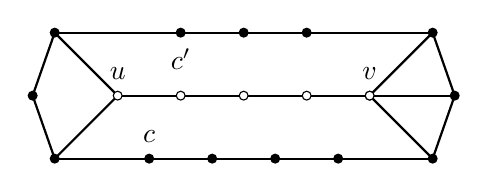
\begin{tikzpicture}[scale=0.8]
    
    
    
    \filldraw (-1,1) circle (2pt);
    \filldraw (-1,-1) circle (2pt);
    \filldraw (-1.35,0) circle (2pt);
    
    \draw[thick] (-1,1) -- (-1.35,0) -- (-1,-1);
    \draw[thick] (0,0) -- (-1,1);
    \draw[thick] (0,0) -- (-1,-1);
    \draw[thick] (5,1) -- (-1,1);
    \filldraw (1,1) circle (2pt);
    \filldraw (2,1) circle (2pt);
    \filldraw (3,1) circle (2pt);
    
    \filldraw (0.5,-1) circle (2pt);
    \filldraw (1.5,-1) circle (2pt);
    \filldraw (2.5,-1) circle (2pt);
    \filldraw (3.5,-1) circle (2pt);
    % \filldraw (3,1) circle (2pt);
    
    \filldraw (5,1) circle (2pt);
    \filldraw (5,-1) circle (2pt);
    \filldraw (5.35,0) circle (2pt);
    
    \draw[thick] (5,1) -- (5.35,0) -- (5,-1);
    \draw[thick] (4,0) -- (5,1);
    \draw[thick] (4,0) -- (5,-1);
    \draw[thick] (4,0) -- (5.35,0);
    
    \draw[thick] (5,-1) -- (-1,-1);
    
    \filldraw (4,0) circle (2pt);
    
    \draw[thick] (0,0) -- (4,0);
        
    \draw[fill=white, draw=black] (2,0) circle (2pt); 
    \draw[fill=white, draw=black] (3,0) circle (2pt);
    \draw[fill=white, draw=black] (0,0) circle (2pt);\node[above] at (0,0.1) {$u$};
    \draw[fill=white, draw=black] (1,0) circle (2pt);
    \draw[fill=white, draw=black] (4,0) circle (2pt);\node[above] at (4,0.1) {$v$};

    \node[above] at (0.5,-0.9) {$c$};
    \node[below] at (1,0.9) {$c'$};


    \end{tikzpicture}
    \caption{An example of a $4$-fat turtle. Let $C$ be the cycle induced by the black vertices, $P$ be the path induced by the white vertices. Then the tuple $(4,C,P,c,c')$ {defines} a $4$-fat turtle.
    % \ff{Can you place $P$, $C$, $u,v$, $c$, $c'$ on the figure?}
    }
    \label{fig:turtle}
\end{figure}


\begin{definition}
For an integer $t\geq 1$, a ``$t$-fat turtle'' consists of a cycle $C$ and an induced $(u,v)$-path $P$ of length at least $t$ 
% \todo{F: at least $t$?} 
such that all of the following hold: 
\begin{enumerate*}[label=(\alph*)]

\item $V(P) \cap V(C) = \emptyset$,

\item For any vertex $w\in (V(P)\setminus \{u,v\})$, $N(w) \cap V(C) = \emptyset$ and both $u$ and $v$ have at least one neighbour in $C$,

\item For any vertex $w\in N(u) \cap V(C)$ and $w'\in N(v)\cap V(C)$, the distance between $w$ and $w'$ in $C$ is at least $t$,

\item There exist two vertices $\{c,c'\}\subset V(C)$ and two distinct components $C_u,C_v$ of $C-\{c,c'\}$ such that $N(u) \cap V(C) \subseteq V(C_u)$ and $N(v) \cap V(C) \subseteq V(C_v)$.

\end{enumerate*}

The tuple $(t,C,P,c,c')$ defines the $t$-fat turtle. See Figure~\ref{fig:turtle} for an example.
\end{definition}

In the following observation, we show that any ($t$-theta, $t$-pyramid,$t$-prism)-free graph cannot contain a $(t+1)$-fat turtle as an induced subgraph.

\begin{lemma}\label{lem:fat-turtle}
For some integer $t\geq 1$, let $G$ be a graph containing a $(t+1)$-fat turtle as an induced subgraph. Then $G$ is not ($t$-theta, $t$-pyramid, $t$-prism)-free.  
\end{lemma}
 \begin{proof}
 Let $(t+1,C,P,c,c')$ be a $(t+1)$-fat turtle in $G$. Let the vertices of $C$ be named $c=a_0, a_1, \ldots, a_k=c', a_{k+1},\ldots, a_{|V(C)|}$ as they are encountered while traversing $C$ starting from $c$ in a counter-clockwise manner. Denote by
 $u,v$ the end-vertices of $P$. By definition, there exist two distinct components $C_u,C_v$ of $C-\{c,c'\}$ such that $N(u) \cap V(C) \subseteq V(C_u)$ and $N(v) \cap V(C) \subseteq V(C_v)$. Without loss of generality, assume $V(C_u) = \{a_1, a_2, \ldots, a_{k-1}\}$ and $V(C_v) = \{a_{k+1}, a_{k+2}, \ldots, a_{|V(C)|}\}$. Let $i^-$ and $i^+$ be the minimum and maximum indices such that $a_{i^-}$ and $a_{i^+}$ are adjacent to $u$. Let $j^-$ and $j^+$ be the minimum and maximum indices such that $a_{j^-}$ and $a_{j^+}$ are adjacent to $v$. By definition, $i^-\leq i^+ < j^-\leq j^+$. Let $P_1$ be the $(a_{i^-},a_{j^+})$-subpath of $C$ containing $c$. Let $P_2$ be the $(a_{i^+},a_{j^-})$-subpath of $C$ that contains $c'$. Observe that $P_1$ and $P_2$ have length at least $t$ (by definition). Now we show that $P,P_1,P_2$ together form one of theta, pyramid or prism. If $a_{i^-} = a_{i^+}$ and $a_{j^-} = a_{j^+}$, then $P,P_1,P_2$ form a $t$-theta. If $i^-\leq i^+-2$ and $j^-\leq j^+-2$, then also $P,P_1,P_2$ form a $t$-theta. If $j^-= j^+-1$ and $i^-= i^+-1$, then $P,P_1,P_2$ form a $t$-prism. In any other case, $P,P_1,P_2$ form a $t$-pyramid.
 \end{proof}



In the remainder of this section, we shall prove that there exists a linear function $f(t)$ such that if the isometric path antichain cover number of a graph is more than $f(t)$, then $G$ is forced to contain a $(t+1)$-fat turtle as an induced subgraph, and therefore is not ($t$-theta, $t$-pyramid,$t$-prism)-free. We shall use the following observation.


%  \begin{definition}
%  An induced cycle $C$ with $t\geq 4$ of a graph $G$ is ``\emph{fat}" if there exist two non-adjacent vertices $u,v\in V(C)$ and an induced $(u,v)$-path $P$ in $G$ such that all of the following holds:
%  \begin{enumerate}[label=(\alph*)]
%  \item There exists a $(u',v')$-subpath $P'$ of $P$ with $V(P')\cap V(C)=\{u',v'\}$.
%  \item Let $u_1$ (resp. $v_1$) be the neighbour of $u'$ (resp. $v'$) in $P'$. Then $N[u_1]\cap N[v_1]\subseteq V(P')$ and for any vertex $w\in V(P')\setminus \{u',v',u_1,v_1\}$, $N[w]\cap V(C)=\emptyset$ 

%  \item There exists a vertex $t\in V(C)$ such that, in a counterclockwise traversal of $C$ starting from $t$, all vertices in $N[u_1]\cap V(C)$ appears before those in $N[v_1]\cap V(C)$.
%  \end{enumerate}
%  The path $P$ is the ``\emph{connector path}''.
% \end{definition}



\begin{observation}\label{obs:anti-cp-reduc}
\sloppy Let $G$ be a graph, $r$ be an arbitrary vertex, $P$ be an isometric $(u,v)$-path in $G$ and $Q$ be a subpath of an isometric $(v,r)$-path in $G$ such that one endpoint of $Q$ is $v$. Let $P'$ be the maximum $(u,w)$-subpath of $P$ such that no internal vertex of $P'$ is a neighbour of some vertex of $Q$. We have that $|\anticp{r}{P'}| \geq |\anticp{r}{P}| - 3$. 
\end{observation}

 \begin{proof}
 Suppose $|\anticp{r}{P'}| \leq |\anticp{r}{P}| - 4$ and consider the $(w,v)$-subpath, say $P''$, of $P$. Observe that $|\anticp{r}{P''}| \geq 4$. Now let $w'$ be a vertex of $Q$ which is a neighbour of $w$. Observe that $|\dist{r}{w} - \dist{r}{w'}| \leq 1$ and therefore $\dist{w}{v} = |E(P'')| \leq |\dist{r}{w} - \dist{r}{v}| + 2 $. But this contradicts Proposition~\ref{prp:antichain-length}, which implies that the length of $P''$ is at least $|\dist{r}{w} - \dist{r}{v}| + 3$.
 \end{proof}


%\vspace{-10pt}
% For technical purpose, we shall also need the following definition.


%  \begin{definition}\label{def:top-path}
%  Let $G$ be a graph and $r$ be an arbitrary vertex. An induced $(u,v)$-path 
%  $P$ is a ``\emph{top $(u,v)$-path} with respect to $r$'' if $P$ can be partitioned into two subpaths $P_u$ and $P_v$ such that all of the following holds.
%  \begin{enumerate}
 
%     % \item For all vertices, $w\in V(P)\setminus \{u,v\}$ $\dist{r}{w} < \dist{r}{u}$.
    
%      \item The vertex $u$ is one of the end-vertices of $P_u$ and there is an isometric $(u,r)$-path $Q_u$ such that $P_u$ is a subpath of $Q_u$.
     
%      \item The vertex $v$ is one of the end-vertices of $P_v$ and there is an isometric $(v,r)$-path $Q_v$ such that $P_v$ is a subpath of $Q_v$.
%  \end{enumerate}
%  \end{definition}

% % The next observation follows immediately from Definition~\ref{def:top-path} and the definition of $\overrightarrow{G_r}$.

% % \begin{observation}\label{obs:top-path}
% % Let $r$ be an arbitrary vertex of $G$ and $u,v$ be two non-adjacent vertices such that $\dist{r}{u}=\dist{r}{v}$. Let $Q_u$ (resp. $Q_v$) be an isometric $(u,r)$-path (resp. isometric $(v,r)$-path) in $G$. Then there exists a top path $T$ between $u$ and $v$ with respect to $r$ such that $V(T) \subseteq V(Q_u) \cup V(Q_v)$.
% % \end{observation}

\newcommand{\vertical}[2]{Q\left({#1},{#2}\right)}



\begin{figure}[t]
\centering
    \scalebox{0.9}{
    \centering
    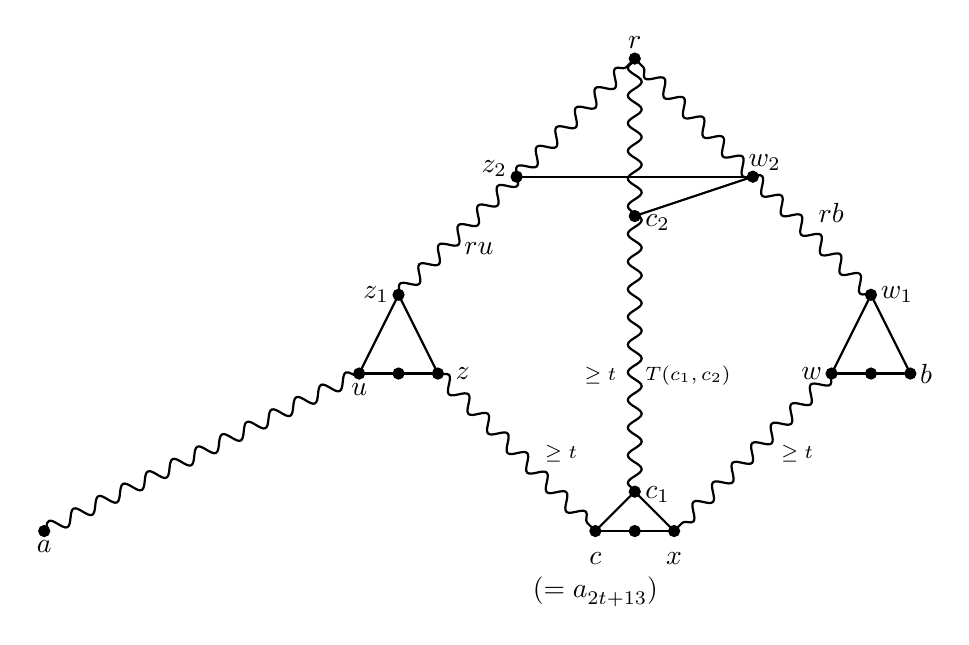
\begin{tikzpicture}
    
    \filldraw (3.5,4) circle (2pt);
    \node[above] at (3.5,4) {$r$};
    \filldraw (3.5,2) circle (2pt);
    \filldraw (5,2.5) circle (2pt);
    \filldraw (2,2.5) circle (2pt);
    \node[left] at (2,2.6) {$z_2$};
    \node[above] at (5.15,2.45) {$w_2$};
    
    
    \draw[thick] (2,2.5) -- (5,2.5);
    \draw[thick] (3.5,2) -- (5,2.5);
    
    
    \filldraw (0,0) circle (2pt);
    \node[below] at (0,0) {$u$};
    
    \filldraw (0.5,0) circle (2pt);
    \filldraw (1,0) circle (2pt);
    \node[right] at (1.1,0) {$z$};
    
    \draw[thick] (0,0) -- (1,0);
    \draw[thick] (0,0) -- (0.5,1) -- (1,0);
    
    
    \filldraw (0.5,1) circle (2pt);
    \node[left] at (0.5,1) {$z_1$};
    
    
    \filldraw (6,0) circle (2pt);
    \node[left] at (6,0) {$w$};
    \filldraw (6.5,0) circle (2pt);
    \filldraw (7,0) circle (2pt);
    \node[right] at (7,0) {$b$};
    
    \draw[thick] (6,0) -- (7,0);
    \node[right] at (6.5,1) {$w_1$};
    \draw[thick] (6,0) -- (6.5,1) -- (7,0);
    
    \filldraw (6.5,1) circle (2pt);
    \filldraw (3.5,-1.5) circle (2pt);
    
    
    \filldraw (3,-2) circle (2pt);
    \filldraw (3.5,-2) circle (2pt);
    \filldraw (4,-2) circle (2pt);
    \node[below] at (3,-2) {\begin{tabular}{c}
         $c$ \\ $(= a^{}_{2t+13})$ 
    \end{tabular}};
    \node[below] at (4,-2) {\begin{tabular}{c} $x$ \end{tabular}};
    
    \draw[thick] (3,-2) -- (4,-2);
    
    \draw[thick] (3,-2) -- (3.5,-1.5) -- (4,-2) ;
    \node[right] at (3.3,-1.5) {\begin{tabular}{c}
         $c_1$ 
    \end{tabular}};
    
    \filldraw (-4,-2) circle (2pt);
    \node[below] at (-4,-2) {$a$};
    \node[right] at (3.3,1.95) {\begin{tabular}{c}
         $c_2$ 
    \end{tabular}};
    
    \node[right] at (3.3,0) {\begin{tabular}{c}
         \scriptsize $T(c_1,c_2)$ 
    \end{tabular}};
    \node[left] at (3.6,0) {\begin{tabular}{c}
         \scriptsize $\geq t$ 
    \end{tabular}};
    
    
    \node[left] at (6.1,-1) {\begin{tabular}{c}
         \scriptsize $\geq t$ 
    \end{tabular}};
    
    
    \node[left] at (3.1,-1) {\begin{tabular}{c}
         \scriptsize $\geq t$ 
    \end{tabular}};
    
    \path [draw=black, thick,snake it] (-4,-2) -- (0,0);
    \path [draw=black, thick,snake it] (1,0) -- (3,-2);
    \path [draw=black, thick,snake it] (6,0) -- (4,-2);
    \path [draw=black, thick,snake it] (0.5,1) -- (3.5,4);
    \path [draw=black, thick,snake it] (6.5,1) -- (3.5,4);
    \path [draw=black, thick, snake it] (3.5,-1.5) -- (3.5,2) -- (3.5,4);
    
    \node[right] at (5.5,2) {\begin{tabular}{c}
          $\vertical{r}{b}$ 
    \end{tabular}};
    
    \node[right] at (1, 1.6) {\begin{tabular}{c}
         $\vertical{r}{u}$ 
    \end{tabular}};
    
    \end{tikzpicture}}
    \caption{Illustration of the notations used in the proof of Lemma~\ref{lem:ipac-fat}.}\label{fig:proof-illustrate}
\end{figure}

\begin{lemma}\label{lem:ipac-fat}
For an integer $t\geq 1$, let $G$ be a graph with $\ipac{G}\geq 8t+64$. Then $G$ has a $(t+1)$-fat turtle {as an induced subgraph}.
\end{lemma}

\begin{proof}


Let $r$ be a vertex of $G$ such that $\ipac{\overrightarrow{G_r}}$ is at least $8t+64$. Then there exists an isometric path $P$ such that $|\anticp{r}{P}|\geq 8t+64$. Let the two endpoints of $P$ be $a$ and $b$. (See Figure~\ref{fig:proof-illustrate}.) Let $u$ be a vertex of $P$ such that $\dist{r}{u}=\dist{r}{P}$. Let $\Pnote{a}{u}$ be the $(a,u)$-subpath of $P$ and $\Pnote{b}{u}$ be the $(b,u)$-subpath of $P$. Both $\Pnote{a}{u}$ and $\Pnote{b}{u}$ are isometric paths and observe that either $|\anticp{r}{\Pnote{a}{u}}|\geq 4t+32$ or  $|\anticp{r}{\Pnote{b}{u}}|\geq 4t+32$. Without loss of generality, assume that  $|\anticp{r}{\Pnote{b}{u} }|\geq 4t+32$. Let $\vertical{r}{b}$ be an isometric $(b,r)$-path in $G$. First observe that $u$ is not adjacent to any vertex of $\vertical{r}{b}$. Otherwise, $\dist{u}{b} \leq 2 + \dist{r}{b}-\dist{r}{u}$, which contradicts Proposition~\ref{prp:antichain-length}. Let $\Pnote{u}{w}$ be the maximum $(u,w)$-subpath, of $\Pnote{b}{u}$ such that no internal vertex of $\Pnote{u}{w}$ is a neighbour of $\vertical{r}{b}$. Note that $\Pnote{u}{w}$ is an isometric path and $w$ has a neighbour in $\vertical{r}{b}$. Applying Observation~\ref{obs:anti-cp-reduc}, we have the following:

\begin{claim}
$|\anticp{r}{\Pnote{u}{w}}| \geq 4t+29$.
\end{claim}

Let $\vertical{r}{u}$ be any isometric $(u,r)$-path of $G$. Observe that $w$ is not adjacent to any vertex of $\vertical{r}{u}$. Otherwise, $\dist{u}{w} \leq 2 + \dist{r}{u}-\dist{r}{w}$, which contradicts Proposition~\ref{prp:antichain-length}.  Let $\Pnote{z}{w}$ be the maximum $(z,w)$-subpath of $\Pnote{u}{w}$ such that no internal vertex of $\Pnote{z}{w}$ has a neighbour in $\vertical{r}{u}$. Observe that $\Pnote{z}{w}$ is an isometric path, and $z$ has a neighbour in $\vertical{r}{u}$. Again applying Observation~\ref{obs:anti-cp-reduc}, we have the following:

\begin{claim}\label{cl:2}
$|\anticp{r}{\Pnote{z}{w}}| \geq 4t+26$.
\end{claim}


Let $a_1, a_2, \ldots,a_k$ be the vertices of $\anticp{r}{\Pnote{z}{w}}$ ordered according to their appearance while traversing $\Pnote{z}{w}$ from $z$ to $w$. Due to Claim~\ref{cl:2}, we have that $k\geq 4t+26$. Let $c=a_{2t+13}$ and $\vertical{r}{c}$ denote an isometric $(c,r)$-path. Let $T(r,c_1)$ 
be the maximum subpath of $\vertical{r}{c}$ such that no internal vertex of $T(r,c_1)$ is adjacent to any vertex of $\Pnote{z}{w}$. Observe that neither $z$ nor $w$ can be adjacent to $c_1$ (due to Proposition~\ref{prp:antichain-length}). Morevoer, if $c_1$ is a vertex of $\Pnote{z}{w}$ then we must have $c_1=c$.

\begin{claim}\label{clm:life-saver}
Let $x$ be a neighbour of $c_1$ in $\Pnote{z}{w}$, $X$ be the $(x,b)$-subpath of $\Pnote{u}{b}$ and $Y$ be the $(x,u)$-subpath of $\Pnote{u}{b}$. Then $|\anticp{r}{X}| \geq 2t+11$ and $|\anticp{r}{Y}| \geq 2t+11$.
\end{claim}


 \begin{proof}
\sloppy  Let $\Pnote{c}{w}$ denote the %subpath of 
 $(c,w)$-subpath of $\Pnote{z}{w}$. Observe that $|\anticp{r}{\Pnote{c}{w}}| \geq 2t+14$.
 First, consider the case when $x$ lies in the $(z,c)$-subpath of $\Pnote{z}{w}$. In this case, $\Pnote{c}{w}$ is a subpath of $X$ and therefore $|\anticp{r}{X}| \geq 2t+14$. Now consider the case when $x$ lies in $\Pnote{c}{w}$. In this case, applying Observation~\ref{obs:anti-cp-reduc}, we have that $|\anticp{r}{X}| \geq |\anticp{r}{\Pnote{c}{w}}| - 3 \geq 2t+11$. Using a similar argument, we have that $|\anticp{r}{Y}| \geq 2t+11$.
 \end{proof}

Let $T(c_1,c_2)$ be the maximum $(c_1,c_2)$-subpath of $T(c_1,r)$ such that no internal vertex of $T(c_1,c_2)$ is adjacent to a vertex of $\vertical{r}{b}$ or $\vertical{r}{u}$. {Note that, if $c_2$ lies on $\vertical{r}{b}$ or $\vertical{r}{u}$, we must have $c_2=r$}.  We have the following claim.

 \begin{claim}\label{clm:vacant-path}
 The length of $T(c_1,c_2)$ is at least $t+3$.
 \end{claim}

  \begin{proof}
 Assume that the length of $T(c_1,c_2)$ is at most $t+2$ and $x$ be a neighbour of $c_1$ in $\Pnote{z}{w}$. Observe that all vertices of $\Pnote{z}{w}$ are at distance at least $\dist{r}{u}$ \textit{i.e.} $\dist{r}{\Pnote{z}{w}} \geq \dist{r}{u}$, {since $\dist{r}{u}=\dist{r}{P}$}. Hence, 

 \medskip \textbf{(+)} $\dist{r}{x} \geq \dist{r}{u}$ and $\dist{r}{c_1} \geq \dist{r}{u} - 1$.

\noindent Now, suppose $c_2$ has a neighbour $c_3$ in $\vertical{r}{u}$. Hence $\dist{c_3}{x} \leq \dist{c_3}{c_2} + \dist{c_2}{c_1} + \dist{c_1}{x} \leq t+4$. Now, using (+) and the fact that $c_3$ lies on an isometric $(r,u)$-path ($\vertical{r}{u}$), we have that $\dist{c_3}{u} \leq t+4$. Therefore, $\dist{u}{x} \leq \dist{c_3}{u} + \dist{c_3}{x} \leq 2t+8$.  But this contradicts  Proposition~\ref{prp:antichain-length} and Claim~\ref{clm:life-saver}, as they together imply that $\dist{u}{x}$ is at least $\dist{r}{x} - \dist{r}{u} + 2t+10 {\geq 2t+10}$.


 Hence, $c_2$ must have a neighbour $c_3$ in $\vertical{r}{b}$. First, assume that $\dist{r}{x} \geq \dist{r}{b}$. Then, as $\dist{c_3}{x} \leq \dist{c_3}{c_2} + \dist{c_2}{c_1} + \dist{c_1}{x} \leq t+4$ and $c_3$ lies on an isometric $(r,b)$-path ($\vertical{r}{b}$), we have that $\dist{x}{b} \leq 2t+8$. But {again} this contradicts  Proposition~\ref{prp:antichain-length} and Claim~\ref{clm:life-saver}, as they together imply that the length of $\dist{x}{b}$ is at least $\dist{r}{x} - \dist{r}{u} + 2t+10$. Now, assume that $\dist{r}{x} < \dist{r}{b}$. Let $b'$ be a vertex of $\vertical{r}{b}$ such that $\dist{r}{b'} = \dist{r}{x}$. Using a similar argumentation as before, we have that $\dist{x}{b'} \leq 2t+8$. Hence, $\dist{x}{b} \leq \dist{x}{b'} + \dist{b'}{b} \leq \dist{r}{b} - \dist{r}{x} + 2t+8$.
% % \todo{F: I don't understand where this last one comes from... \dd{Is it clear now?} yes} 
 But this contradicts Proposition~\ref{prp:antichain-length} which, due to Claim~\ref{clm:life-saver}, implies that $\dist{x}{b} \geq \dist{r}{b} - \dist{r}{x} + 2t+10$.
 \end{proof}

The path $T(c_1,c_2)$ forms the first ingredient to extract a $(t+1)$-fat turtle. Let $z_1$ be the neighbour of $z$ in $\vertical{r}{u}$ and $w_1$ be the neighbour of $w$ in $\vertical{r}{b}$. We have the following claim.

\begin{claim}\label{clm:final}
The vertices $w_1$ and $z_1$ are non adjacent.
\end{claim}

 \begin{proof}
 Recall that $z_1$ lies in $\vertical{r}{u}$ and $\dist{r}{z} \geq \dist{r}{u}$. Hence $z_1$ must be a neighbour of $u$. If $w_1$ and $z_1$ are adjacent, then observe that $\dist{u}{b} \leq \dist{r}{b} - \dist{r}{w_1} + 2 \leq $. This implies $\dist{u}{b} \leq \dist{r}{b} - \dist{r}{u} + 3$. But this shall again contradict Proposition~\ref{prp:antichain-length}.
 \end{proof}

Now we shall construct a $(w_1,z_1)$-path as follows: Consider the maximum $(w_1,w_2)$-subpath, say $T(w_1,w_2)$, of $\vertical{r}{b}$ such that no internal vertex of $T(w_1,w_2)$ has a neighbour in $\vertical{r}{u}$. Similarly, consider the maximum $(z_1,z_2)$-subpath, say $T(z_1,z_2)$, of $\vertical{r}{u}$ such that no internal vertex of $T(z_1,z_2)$ is a neighbour of $w_2$. {(Note that it is possible that $z_2=w_2=r$.)}
% \todo{F: something wrong in that previous sentence.}
Let $T$ be the path obtained by taking the union of $T(w_1,w_2)$ and $T(z_1,z_2)$. Observe that $z_2$ must be a neighbour of $w_2$ and $T$ is an induced $(w_1,z_1)$-path. The definitions of $T$ and $\Pnote{z}{w}$ imply that their union induces a cycle $Z$. Here we have the second and final ingredient to extract the $(t+1)$-fat turtle.

Suppose that $c_2$ has a neighbour in $T$. Let $T'$ be the maximum subpath of $T(c_1,c_2)$ which is vertex-disjoint
% \todo{F: by the definition of $T(c_1,c_2)$, I think the whole path is vertex-disjoint from $Z$, since no internal vertex is adjacent to a vertex of it?}
from $Z$. ({Note that if $c_1=c$ or $c_2\in \{w_2,z_2\}$ (e.g. when $c_2=w_2=z_2=r$), $T(c_1,c_2)$ may share vertices with $Z$}.) Due to Claim~\ref{clm:vacant-path}, the length of $T'$ is at least $t+1$. Let $e_1$ and $e_2$ be the end-vertices of $T'$. Observe the following.

\begin{itemize}
    \item Each of $e_1$ and $e_2$ has at least one neighbour in $Z$.
    
    \item $Z-\{z,w\}$ contains two distinct components $C_1,C_2$ such that for $i\in \{1,2\}$, $N(e_i)\cap V(Z) \subseteq V(C_i)$.
    
    \item For a vertex $e_1'\in N(e_1)\cap V(Z)$ and $e_2'\in N(e_2)\cap V(Z)$, the distance between $e'_1$ and $e'_2$ is at least $t+1$. This statement follows from Claim~\ref{clm:life-saver}.
\end{itemize}

Hence, we have that the tuple $(t+1,Z,T',z,w)$ defines a $(t+1)$-fat turtle. Now consider the case when $c_2$ does not have a neighbour in $T$. By definition, $c_2$ has at least one neighbour in $\vertical{r}{u}$ or $\vertical{r}{b}$. Without loss of generality, assume that $c_2$ has a neighbour $c_3$ in $\vertical{r}{u}$ such that the $(z_2,c_3)$-subpath, say, $T''$ of $\vertical{r}{u}$ has no neighbour of $c_2$ {other than $c_3$}. Observe that the path $T^*= (T' \cup (T''-\{z_2\}))$ is vertex-disjoint from $Z$ and has length at least $t+1$. Let $e_1,e_2$ be the two end-vertices of $T^*$. Observe the following.
\begin{itemize}
    \item Each of $e_1$ and $e_2$ has at least one neighbour in $Z$.
    
    \item $Z-\{z,w\}$ contains two distinct components $C_1,C_2$ such that for $i\in \{1,2\}$, $N(e_i)\cap V(Z) \subseteq V(C_i)$.
    
    \item For a vertex $e_1'\in N(e_1)\cap V(Z)$ and $e_2'\in N(e_2)\cap V(Z)$, the distance between $e'_1$ and $e'_2$ is at least $t+1$. This statement follows from Claim~\ref{clm:life-saver}.
\end{itemize}

 Hence, $(t+1,Z,T^*,z,w)$ is a $(t+1)$-fat turtle
\end{proof}



\noindent \textbf{Proof of Theorem~\ref{thm:main}\ref{thm:truemper}:} Lemma~\ref{lem:ipac-ipco}, \ref{lem:fat-turtle} and~\ref{lem:ipac-fat} together imply Theorem~\ref{thm:main}\ref{thm:truemper}.



% \section{Proof of Theorem~\ref{thm:outer}}\label{sec:outer}

% Next, we shall show that outerstring graphs are ($4$-theta, $4$-prism, $4$-pyramid)-free.


 \begin{lemma}\label{lem:outer-truemper}
 Any outerstring graph is ($4$-theta, $4$-prism, $4$-pyramid)-free.
 \end{lemma}

    
  \begin{proof}
 To prove the lemma, we shall need to recall a few definitions and results from the literature. A graph $G$ is a \emph{string} graph if there is a collection $S$ of simple curves on the plane and a bijection between $V(G)$ and $S$ such that two curves in $S$ intersect if and only if the corresponding vertices are adjacent in $G$. Let $G$ be a graph with an edge $e$. The graph $G/ e$ is obtained by \emph{contracting} the edge $e$ into a single vertex. Observe that string graphs are closed under edge contraction~\cite{kratochvil1991string}. We shall use the following result.

 \begin{proposition}[\cite{kratochvil1991string}]\label{prp:contract}
 Let $G$ be an outerstring graph with an edge $e$. Then $G/ e$ is an outerstring graph.
 \end{proposition}

  A \emph{full subdivision} of a graph is a graph obtained by replacing each edge of $G$ with a new path of length at least~2.  We shall use the following result implied from Theorem $1$ of~\cite{kratochvil1991string}. 
% % \todo{F: what do you mean by "folklore"? If this is already mentioned somewhere, it would be good to cite it. Same with the other one. {Done}}

 \begin{proposition}[\cite{kratochvil1991string}]\label{prp:k33}
 Let $G$ be a string graph. Then $G$ does not contain a full subdivision of $K_{3,3}$ as an induced subgraph.
 \end{proposition}

 For a graph $G$, the graph $G^+$ is constructed by introducing a new \emph{apex} vertex $a$ and connecting $a$ with all vertices of $G$ by new copies of paths of length at least $2$. We shall use the following result of Biedl \textit{et al.}~\cite{biedl2018size}.


 \begin{proposition}[Lemma 1, \cite{biedl2018size}] \label{prp:apex-string}
 A graph $G$ is an outerstring graph if and only if $G^+$ is a string graph.
 \end{proposition}

 Now we are ready to prove the lemma. Let $G$ be an outerstring graph. Assume for the sake of contradiction that $G$ contains an induced subgraph $H$ which is a $4$-theta, $4$-pyramid, or a $4$-prism. Since every induced subgraph of an outerstring graph is also an outerstring graph, we have that $H$ is an outerstring graph. Let $E$ be the set of edges of $H$ whose both endpoints are part of some triangle. Now consider the graph $H_1= H / E$ which is obtained by contracting all edges in $E$. By Proposition~\ref{prp:contract}, $H_1$ is an outerstring graph and it is easy to check that $H_1$ is a $3$-theta.
 % \todo{F: you mean 3-theta, I think? {Yes. You are right.}} 
 Let $u$ and $v$ be the vertices of $H_1$ with degree~3 and $w_1,w_2,w_3$ be the set of mutually non-adjacent vertices such that for each $i\in \{1,2,3\}$ $\dist{u}{w_i}=2$ and $\dist{v}{w_i}\geq 2$. Since $H_1$ is a $3$-theta, $w_1,w_2,w_3$ exist. Now consider the graph $H_1^+$ and $a$ be the new apex vertex. Due to Proposition~\ref{prp:apex-string}, we have that $H_1^+$ is a string graph. But notice that, for each pair of vertices in $\{x,y\} \subset \{w_1,w_2,w_3,u,v,a\}$, there exists a unique path of length {at least 2} connecting $x,y$. This implies that $H_1^+$ (which is a string graph) contains a full subdivision of $K_{3,3}$, which contradicts Proposition~\ref{prp:k33}. 
  \end{proof}


\noindent \textbf{Proof of Theorem~\ref{thm:main}\ref{thm:outer}:} Lemma~\ref{lem:ipac-ipco}, \ref{lem:fat-turtle}, \ref{lem:ipac-fat}, and~\ref{lem:outer-truemper} together imply Theorem~\ref{thm:main}\ref{thm:outer}.

 

\section{Proof of Theorem~\ref{thm:lower}}\label{sec:lower}

\newcommand{\Graph}[1]{X_{#1}}
\newcommand{\BGraph}[1]{Y_{#1}}
\newcommand{\CGraph}[1]{Z_{#1}}
\newcommand{\DGraph}[1]{W_{#1}}

\begin{figure}
    \centering
    \scalebox{1}{
    \begin{tabular}{cccc}
       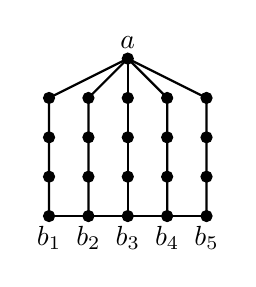
\begin{tikzpicture}
       \filldraw (0,0) circle (2pt);
       \filldraw (0,-0.5) circle (2pt);
       \filldraw (0,-1) circle (2pt);
       \filldraw (0,-1.5) circle (2pt);
       \filldraw (0,-2) circle (2pt);
       
    \filldraw (-0.5,-0.5) circle (2pt);
    \filldraw (-0.5,-1) circle (2pt);
    \filldraw (-0.5,-1.5) circle (2pt);
    \filldraw (-0.5,-2) circle (2pt);
    
    \filldraw (-1,-0.5) circle (2pt);
    \filldraw (-1,-1) circle (2pt);
    \filldraw (-1,-1.5) circle (2pt);
    \filldraw (-1,-2) circle (2pt);
    
    \filldraw (0.5,-0.5) circle (2pt);
    \filldraw (0.5,-1) circle (2pt);
    \filldraw (0.5,-1.5) circle (2pt);
    \filldraw (0.5,-2) circle (2pt);
    
    \filldraw (1,-0.5) circle (2pt);
    \filldraw (1,-1) circle (2pt);
    \filldraw (1,-1.5) circle (2pt);
    \filldraw (1,-2) circle (2pt);
    
    \draw[thick] (0,0) -- (0.5,-0.5) -- (0.5,-2);
    \draw[thick] (0,0) -- (-0.5,-0.5) -- (-0.5,-2);
    \draw[thick] (0,0) -- (-1,-0.5) -- (-1,-2);
    \draw[thick] (0,0) -- (1,-0.5) -- (1,-2);
    \draw[thick] (0,0) -- (0,-0.5) -- (0,-2);
    \draw[thick] (-1,-2) -- (1,-2);
    
    \node[above] at (0,0) {$a$};
    \node[below] at (-1,-2) {$b_1$};    
    \node[below] at (-0.5,-2) {$b_2$};    
    \node[below] at (0,-2) {$b_3$};    
    \node[below] at (0.5,-2) {$b_4$};    
    \node[below] at (1,-2) {$b_5$};
    
       \end{tikzpicture}  & 
       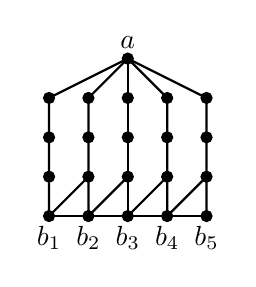
\begin{tikzpicture}
       \filldraw (0,0) circle (2pt);
       \filldraw (0,-0.5) circle (2pt);
       \filldraw (0,-1) circle (2pt);
       \filldraw (0,-1.5) circle (2pt);
       \filldraw (0,-2) circle (2pt);
       
    \filldraw (-0.5,-0.5) circle (2pt);
    \filldraw (-0.5,-1) circle (2pt);
    \filldraw (-0.5,-1.5) circle (2pt);
    \filldraw (-0.5,-2) circle (2pt);
    
    \filldraw (-1,-0.5) circle (2pt);
    \filldraw (-1,-1) circle (2pt);
    \filldraw (-1,-1.5) circle (2pt);
    \filldraw (-1,-2) circle (2pt);
    
    \filldraw (0.5,-0.5) circle (2pt);
    \filldraw (0.5,-1) circle (2pt);
    \filldraw (0.5,-1.5) circle (2pt);
    \filldraw (0.5,-2) circle (2pt);
    
    \filldraw (1,-0.5) circle (2pt);
    \filldraw (1,-1) circle (2pt);
    \filldraw (1,-1.5) circle (2pt);
    \filldraw (1,-2) circle (2pt);
    
    \draw[thick] (0,0) -- (0.5,-0.5) -- (0.5,-2);
    \draw[thick] (0,0) -- (-0.5,-0.5) -- (-0.5,-2);
    \draw[thick] (0,0) -- (-1,-0.5) -- (-1,-2);
    \draw[thick] (0,0) -- (1,-0.5) -- (1,-2);
    \draw[thick] (0,0) -- (0,-0.5) -- (0,-2);
    \draw[thick] (-1,-2) -- (1,-2);
    
    \draw[thick] (-1,-2) -- (-0.5,-1.5);
    \draw[thick] (0,-1.5) -- (-0.5,-2);
    \draw[thick] (0,-2) -- (0.5,-1.5);
    \draw[thick] (1,-1.5) -- (0.5,-2);
    
    \node[above] at (0,0) {$a$};
    \node[below] at (-1,-2) {$b_1$};    
    \node[below] at (-0.5,-2) {$b_2$};    
    \node[below] at (0,-2) {$b_3$};    
    \node[below] at (0.5,-2) {$b_4$};    
    \node[below] at (1,-2) {$b_5$};    
    
       \end{tikzpicture} & 
       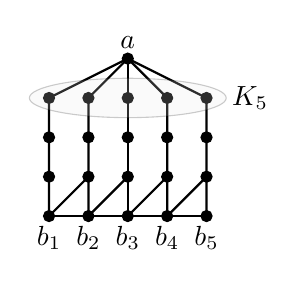
\begin{tikzpicture}
       \filldraw (0,0) circle (2pt);
       \filldraw (0,-0.5) circle (2pt);
       \filldraw (0,-1) circle (2pt);
       \filldraw (0,-1.5) circle (2pt);
       \filldraw (0,-2) circle (2pt);
       
    \filldraw (-0.5,-0.5) circle (2pt);
    \filldraw (-0.5,-1) circle (2pt);
    \filldraw (-0.5,-1.5) circle (2pt);
    \filldraw (-0.5,-2) circle (2pt);
    
    \filldraw (-1,-0.5) circle (2pt);
    \filldraw (-1,-1) circle (2pt);
    \filldraw (-1,-1.5) circle (2pt);
    \filldraw (-1,-2) circle (2pt);
    
    \filldraw (0.5,-0.5) circle (2pt);
    \filldraw (0.5,-1) circle (2pt);
    \filldraw (0.5,-1.5) circle (2pt);
    \filldraw (0.5,-2) circle (2pt);
    
    \filldraw (1,-0.5) circle (2pt);
    \filldraw (1,-1) circle (2pt);
    \filldraw (1,-1.5) circle (2pt);
    \filldraw (1,-2) circle (2pt);
    
    \draw[thick] (0,0) -- (0.5,-0.5) -- (0.5,-2);
    \draw[thick] (0,0) -- (-0.5,-0.5) -- (-0.5,-2);
    \draw[thick] (0,0) -- (-1,-0.5) -- (-1,-2);
    \draw[thick] (0,0) -- (1,-0.5) -- (1,-2);
    \draw[thick] (0,0) -- (0,-0.5) -- (0,-2);
    \draw[thick] (-1,-2) -- (1,-2);
    
    \draw[thick] (-1,-2) -- (-0.5,-1.5);
    \draw[thick] (0,-1.5) -- (-0.5,-2);
    \draw[thick] (0,-2) -- (0.5,-1.5);
    \draw[thick] (1,-1.5) -- (0.5,-2);
    
   \node[above] at (0,0) {$a$};
    \node[below] at (-1,-2) {$b_1$};    
    \node[below] at (-0.5,-2) {$b_2$};    
    \node[below] at (0,-2) {$b_3$};    
    \node[below] at (0.5,-2) {$b_4$};    
    \node[below] at (1,-2) {$b_5$};
    
    \node[right] at (1.2, -0.5) {$K_5$};
    
    \filldraw[fill=gray!20,opacity=0.2,draw=black] (0,-0.5) ellipse (1.25cm and 0.25cm);

       \end{tikzpicture} & 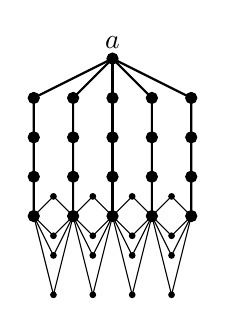
\begin{tikzpicture}
       \filldraw (0,0) circle (2pt);
       \filldraw (0,-0.5) circle (2pt);
       \filldraw (0,-1) circle (2pt);
       \filldraw (0,-1.5) circle (2pt);
       \filldraw (0,-2) circle (2pt);
       
    \filldraw (-0.5,-0.5) circle (2pt);
    \filldraw (-0.5,-1) circle (2pt);
    \filldraw (-0.5,-1.5) circle (2pt);
    \filldraw (-0.5,-2) circle (2pt);
    
    \filldraw (-1,-0.5) circle (2pt);
    \filldraw (-1,-1) circle (2pt);
    \filldraw (-1,-1.5) circle (2pt);
    \filldraw (-1,-2) circle (2pt);
    
    \filldraw (0.5,-0.5) circle (2pt);
    \filldraw (0.5,-1) circle (2pt);
    \filldraw (0.5,-1.5) circle (2pt);
    \filldraw (0.5,-2) circle (2pt);
    
    \filldraw (1,-0.5) circle (2pt);
    \filldraw (1,-1) circle (2pt);
    \filldraw (1,-1.5) circle (2pt);
    \filldraw (1,-2) circle (2pt);
    
    \draw[thick] (0,0) -- (0.5,-0.5) -- (0.5,-2);
    \draw[thick] (0,0) -- (-0.5,-0.5) -- (-0.5,-2);
    \draw[thick] (0,0) -- (-1,-0.5) -- (-1,-2);
    \draw[thick] (0,0) -- (1,-0.5) -- (1,-2);
    \draw[thick] (0,0) -- (0,-0.5) -- (0,-2);
    
    \node[above] at (0,0) {$a$};
    % \node[left] at (-1,-2) {$b_1$};    
    % \node[left] at (-0.5,-2) {$b_2$};    
    % \node[left] at (0,-2) {$b_3$};    
    % \node[left] at (0.5,-2) {$b_4$};    
    % \node[left] at (1,-2) {$b_5$};
     \foreach \x/\y [count = \n] in {-0.75/-1.75,-0.75/-2.25,-0.75/-2.5,-0.75/-3 }
    {
          \filldraw (\x, \y) circle (1pt);
    	 \draw (\x, \y) -- (-1,-2);
          \draw (\x, \y) -- (-0.5,-2);
    }
     \foreach \x/\y [count = \n] in {-0.25/-1.75,-0.25/-2.25,-0.25/-2.5,-0.25/-3 }
    {
          \filldraw (\x, \y) circle (1pt);
    	 \draw (\x, \y) -- (0,-2);
          \draw (\x, \y) -- (-0.5,-2);
    }
    \foreach \x/\y [count = \n] in {0.25/-1.75,0.25/-2.25,0.25/-2.5,0.25/-3 }
    {
          \filldraw (\x, \y) circle (1pt);
    	 \draw (\x, \y) -- (0,-2);
          \draw (\x, \y) -- (0.5,-2);
    }
    \foreach \x/\y [count = \n] in {0.75/-1.75,0.75/-2.25,0.75/-2.5,0.75/-3 }
    {
          \filldraw (\x, \y) circle (1pt);
    	 \draw (\x, \y) -- (1,-2);
          \draw (\x, \y) -- (0.5,-2);
    }
       \end{tikzpicture}\\
         (a) & (b) & (c) & (d) 
    \end{tabular}}
    \caption{(a) $\Graph{4}$~(b) $\BGraph{4}$~(c) $\CGraph{4}$~(d) $\DGraph{4}$.}
    \label{fig:lower}
\end{figure}



{We shall provide a construction for every $k\geq 4$, this implies the statement of Theorem~\ref{thm:lower} for any $k\geq 1$.} 
First we shall prove Theorem~\ref{thm:lower}\ref{it:a}. For a fixed integer $k\geq 4$, first we describe the construction of a graph $\Graph{k}$ as follows. Consider $k+1$ paths $P_1, P_2, \ldots, P_{k+1}$ each of length $k$ and having a common endvertex $a$. For $i\in [k+1]$, let the other endvertex of $P_i$ be denoted as $b_i$. Moreover, for $i\in [k+1]$, let the neighbours of $a$ and $b_i$ in $P_i$ be denoted as $a'_i$ and $b'_i$, respectively. For $i \in [k]$, introduce an edge between $b_i$ and $b_{i+1}$. The resulting graph is denoted $\Graph{k}$ and the special vertex $a$ is the \emph{apex} of $\Graph{k}$. See Figure~\ref{fig:lower}(a). For a fixed integer $k\geq 4$, consider the graph $\Graph{k}$ and for each $i\in [k]$, introduce an edge between $b_i$ and $b'_{i+1}$. Let $\BGraph{k}$ denote the resulting graph and the special vertex $a$ is the \emph{apex} of $\BGraph{k}$. See Figure~\ref{fig:lower}(b). For a fixed integer $k\geq 4$, consider the graph $\BGraph{k}$ and for each $\{i,j\}\subseteq [k]$, introduce an edge between $a'_i$ and $a'_{j}$. Let $\CGraph{k}$ denote the resulting graph and the special vertex $a$ is the \emph{apex} of $\CGraph{k}$. See Figure~\ref{fig:lower}(c). { For a fixed integer $k\geq 4$, consider the graph $\Graph{k}$. For each $i\in [k]$, delete the edge $b_ib_{i+1}$ and introduce $k$ new vertices, each of which is adjacent to only $b_i$ and $b_{i+1}$. Call the resulting graph $W_k$. See Figure~\ref{fig:lower}(d).} 



 We shall use the following result relating hyperbolicity and \emph{isometric cycles}. An induced cycle $C$ of a graph $G$ is \emph{isometric} if for any two vertices $u,v$ of $C$, the distance between $u,v$ in $C$ is the same as that in $G$.

 \begin{proposition}[\cite{wu2011hyperbolicity}]\label{prp:isometric-cycle}
 Let $G$ be a graph containing an isometric cycle of order $k$ with $k \equiv c~(\bmod~4)$. Then the hyperbolicity of $G$ is at least $\lceil\frac{k}{4}\rceil - \frac{1}{2}$ if $c=1$ and $\lceil\frac{k}{4}\rceil$, otherwise.
 \end{proposition}


We now prove the following lemmas.



\begin{lemma}\label{lem:lower-1}
For $k\geq 4$, let $G$ be the graph constructed by taking two distinct copies of $\Graph{k}$ and identifying the two apex vertices. Then $G$ is a (pyramid, prism)-free graph with treewidth $2$, hyperbolicity at least $\lceil\frac{k}{2}\rceil-1$ and $\ipac{G} \geq k$.
\end{lemma}
 \begin{proof}
 Since $G$ is triangle-free, clearly $G$ is (pyramid, prism)-free. Moreover, for any induced cycle $C$ of $G$, and any vertex $w\notin C$, observe that $w$ has only one neighbour in $C$. Therefore, $G$ is also wheel-free. Observe that $G$ has an isometric cycle of length at least $2k$. Therefore, due to Proposition~\ref{prp:isometric-cycle}, $G$ has hyperbolicity at least $\lceil\frac{k}{2}\rceil-1$. Since removing the vertex $a$ from $G$ makes it acyclic, the treewidth of $G$ is two. Let $H$ and $H'$ denote the two copies of $\Graph{k}$ used to construct $G$. Let $r$ be any vertex of $G$ and, without loss of generality, assume that $r$ is a vertex of $H'$. Consider the graph $\overrightarrow{G_r}$. Now recall the construction of $H$ (which is isomorphic to $\Graph{k}$) and consider the path $Q=b_1~b_2\ldots b_k$. Observe that $Q$ is an isometric path and for any two vertices $u,v\in V(Q)$ we have $\dist{r}{u}=\dist{r}{v}$. Therefore, $\anticp{r}{Q} \geq k$. Hence, $\ipac{G} \geq k$. 
 \end{proof}


% Now we shall prove Theorem~\ref{thm:lower}\ref{it:b}.  See Figure~\ref{fig:lower}(b). We prove the following lemma. 


\begin{lemma}\label{lem:lower-2}
For $k\geq 4$, let $G$ be the graph constructed by taking two distinct copies of $\BGraph{k}$ and identifying the two apex vertices. Then $G$ is a (theta, prism)-free graph with treewidth $3$, hyperbolicity at least $\lceil\frac{k}{2}\rceil-1$, and $\ipac{G} \geq k$.
\end{lemma}

 \begin{proof}
 Since removing the special vertex $a$ from $G$ results in a graph with treewidth $2$, it follows that $G$ has treewidth at most $3$. Observe that $G$ has an isometric cycle of length at least $2k$. Therefore, due to Proposition~\ref{prp:isometric-cycle}, $G$ has hyperbolicity at least $\lceil\frac{k}{2}\rceil-1$. Let $H$ and $H'$ denote the two copies of $\BGraph{k}$ used to construct $G$. First we shall show that $H$ does not contain a theta or a prism. Consider the graph $H_1$ obtained by removing the apex of $H$. Observe that $H_1$ does not contain a vertex $v$ such that the vertices in $N[v]$ induce a $K_{1,3}$. Hence $H$ does not contain a theta. It also can be verified that $H_1$ does not contain a prism. Since the neighbourhood of $a$ is triangle-free, it follows that $H$ does not contain a prism. Similarly, $H'$ does not contain a theta or a prism. Now, from our construction, it follows that $G$ does not contain a theta or a prism.  Moreover, for any induced cycle $C$ of $G$, and any vertex $w\notin C$, observe that $w$ has at most two neighbours in $C$. Therefore, $G$ is wheel-free. Using arguments similar to the ones used in the proof of Lemma~\ref{lem:lower-1}, we have that $\ipac{G} \geq k$.   
 \end{proof}




% Now, we shall prove Theorem~\ref{thm:lower}\ref{it:c}.  See Figure~\ref{fig:lower}(c). We prove the following lemma. 


\begin{lemma}\label{lem:lower-3}
For $k\geq 4$, let $G$ be the graph constructed by taking two distinct copies of $\CGraph{k}$ and identifying the two apex vertices. Then $G$ is a (theta, pyramid)-free graph with hyperbolicity at least $\lceil\frac{k}{2}\rceil-1$ and $\ipac{G} \geq k$.
\end{lemma}

 \begin{proof}
 Observe that $G$ has an isometric cycle of length at least $2k$. Therefore, due to Proposition~\ref{prp:isometric-cycle}, $G$ has hyperbolicity at least $\lceil\frac{k}{2}\rceil-1$. Let $H$ and $H'$ denote the two copies of $\BGraph{k}$ used to construct $G$. Observe that $H$ does not contain a vertex $v$ such that the vertices in $N[v]$ induce a $K_{1,3}$. Therefore, $H$ does not contain a theta or a pyramid.  Similarly, $H'$ does not contain a theta or a pyramid. Due to our construction, it follows that $G$ does not contain a theta or a pyramid. Moreover, for any induced cycle $C$ of $G$, and any vertex $w\notin C$, observe that $w$ has at most two neighbours in $C$. Therefore, $G$ is wheel-free. Using arguments similar to the ones used in the proof of Lemma~\ref{lem:lower-1}, we have that $\ipac{G} \geq k$.
 \end{proof}

 {
An isometric path cover $C$ of a graph $G$ is \emph{rooted} if there exists a vertex $v$ such that all paths in $C$ are $v$-rooted isometric paths.

\begin{lemma}\label{lem:lower-4}
For $k\geq 4$, let $G$ be the graph constructed by taking two distinct copies of $\DGraph{k}$ and identifying the two apex vertices. Then $G$ is a (prism, pyramid, wheel)-free planar graph such that any rooted isometric path cover of $G$ has cardinality at least $k^2$ but there is an isometric path cover of $G$ of cardinality $3k+1$.
\end{lemma}

\begin{proof}
      The construction ensures that $G$ is a (prism, pyramid, wheel)-free planar graph. Let $H$ and $H'$ denote the two copies of $\DGraph{k}$ used to construct $G$ and $a$ denote the apex vertex. Observe that there are $k^2$ vertices at maximum distance from the apex vertex $a$ in $H$ and a $a$-rooted isometric path can only cover one of them. Therefore, at least $k^2$ many $a$-rooted isometric paths are needed to cover the graph $H$. As $H'$ is isomorphic to $H$, it has the above properties. Since $a$ is a cut-vertex in $G$, it is easy to verify that for any vertex $v\in V(G)$, any $v$-rooted isometric path cover of $G$ requires $k^2$ many paths. On the other hand, it is easy to check that $G$ has an isometric path cover of cardinality $3k+1$. Indeed $k+1$ geodesics are sufficient to cover the vertices of the maximal isometric paths containing $a$, $2k$ geodesics are sufficient to cover the remaining vertices of $G$.
\end{proof}

}

Lemma~\ref{lem:ipac-ipco}, \ref{lem:lower-1}, \ref{lem:lower-2}, \ref{lem:lower-3}, \ref{lem:lower-4} imply Theorem~\ref{thm:lower}.

% \section{Proof of Theorem~\ref{thm:general-step-1}}\label{sec:general-step-1}
% Let $T$ be a tree-decomposition of a graph $G$. Define $length(T) = \displaystyle\max\limits_{\substack{v\in V(T)\\ u,v\in X_v}} \dist{u}{v}$, where the distance $\dist{u}{v}$ denotes the number of edges in a shortest path between $u$ and $v$ in $G$. The \emph{treelength} of $G$, denoted as $\treelength{G}$, is defined as $\min_T length(T)$, where the minimum is taken over all tree-decompositions of $G$. We shall use the following results.

% \begin{proposition}[\cite{ChakrabortyD0FG22}]
% Let $G$ be a graph with treelength at most $\ell$. Then $\ipac{G} \leq 6\ell+3$.
% \end{proposition}


% \begin{proposition}[\cite{coudert2016approximate}]
% The treelength of any graph $G$ with no isometric cycle of length greater than $c$ is at most $\frac{c}{2}.tw(G)$, where $tw(G)$ is the treewidth of $G$.
% \end{proposition}

% \begin{proposition}[\cite{FloOtherISAAC}]
% Any graph $G$ admitting an isometric path cover of cardinality at most $k$ has treewidth $2^{2^{O(k \log k)}}$.\todo{F: for the full version, we are soon going to post on arXiv a $3^k$ bound.} \todo{D: Nice.}
% % $(2k^2)2^{k+1}k!$.
% \end{proposition}

% When the length of a longest isometric cycle of a graph $G$ is bounded by a constant, the above three propositions together imply that $\ipac{G}$ is $O\left(2^{2^{k \log k}}\right)$ where $k$ is the minimum size of an isometric path cover of $G$. The above observation and Lemma~\ref{lem:ipac-ipco} prove Theorem~\ref{thm:general-step-1}.

\vspace{-5pt}


\section{Conclusion}\label{sec:conclu}

In this paper, we have introduced the new graph parameter \emph{isometric path complexity}. We have shown that the isometric path complexity of a graph with $n$ vertices and $m$ edges can be computed in $O(n^2 m)$-time. It would be interesting to provide a faster algorithm to compute the isometric path complexity of a graph. We have derived upper bounds on the isometric path complexity of three seemingly (structurally) different classes of graphs, namely hyperbolic graphs, (theta,pyramid,prism)-free graphs and outerstring graphs. An interesting direction of research is to generalise the properties of hyperbolic graphs or (theta,pyramid,prism)-free graphs to graphs with bounded isometric path complexity.

Note that, in our proofs we essentially show that, for any graph $G$ that belongs to one of the above graph classes, any vertex $v$ of $G$, and any isometric path $P$ of $G$, the path $P$ can be covered by a small number of $v$-rooted isometric paths. This implies our ``choice of the root'' is arbitrary. This motivates the following definition. The \emph{strong isometric path complexity} of a graph $G$% , denoted by $\ipco{G}$,
is the minimum integer $k$ such that for each vertex $v\in V(G)$ we have that the vertices of any isometric path $P$ of $G$ can be covered by $k$ many $v$-rooted isometric paths. Our proofs imply that the strong isometric path complexity of graphs from all the graph classes addressed in this paper are bounded. 
% It would be interesting to further study properties of graphs with bounded strong isometric path complexity. 
% Another interesting question is to find ``special roots'' that would lead to better bounds on the isometric path complexity of the graph classes addressed in this paper. 
We also wonder whether one can find other interesting graph classes with small (strong) isometric path complexity. 

Our results imply a constant-factor approximation algorithm for \IPC on hyperbolic graphs, (theta, pyramid, prism)-free graphs and outerstring graphs. However, the existence of a constant-factor approximation algorithm for \IPC on general graphs is not known (an $O(\log n)$-factor approximation algorithm is designed in~\cite{TG21}).






\bibliographystyle{plain}
\bibliography{references}


\end{document}

